%===============================================================================
% LaTeX sjabloon voor de bachelorproef toegepaste informatica aan HOGENT
% Meer info op https://github.com/HoGentTIN/latex-hogent-report
%===============================================================================

\documentclass[dutch,dit,thesis]{hogentreport}

% TODO:
% - If necessary, replace the option `dit`' with your own department!
%   Valid entries are dbo, dbt, dgz, dit, dlo, dog, dsa, soa
% - If you write your thesis in English (remark: only possible after getting
%   explicit approval!), remove the option "dutch," or replace with "english".

\usepackage{lipsum} % For blind text, can be removed after adding actual content

%% Pictures to include in the text can be put in the graphics/ folder
\graphicspath{{graphics/}}

%% For source code highlighting, requires pygments to be installed
%% Compile with the -shell-escape flag!
\usepackage[section]{minted}
\usemintedstyle{solarized-light}
\definecolor{bg}{RGB}{253,246,227} %% Set the background color of the codeframe

%% Change this line to edit the line numbering style:
\renewcommand{\theFancyVerbLine}{\ttfamily\scriptsize\arabic{FancyVerbLine}}

%% Macro definition to load external java source files with \javacode{filename}:
\newmintedfile[javacode]{java}{
    bgcolor=bg,
    fontfamily=tt,
    linenos=true,
    numberblanklines=true,
    numbersep=5pt,
    gobble=0,
    framesep=2mm,
    funcnamehighlighting=true,
    tabsize=4,
    obeytabs=false,
    breaklines=true,
    mathescape=false
    samepage=false,
    showspaces=false,
    showtabs =false,
    texcl=false,
}

\lstset{
    language=yaml
    basicstyle=\ttfamily,
    columns=fullflexible,
    frame=single,
    breaklines=true
}
% Other packages not already included can be imported here

%%---------- Document metadata -------------------------------------------------
% TODO: Replace this with your own information
\author{Jurn De Vleeschauwer}
\supervisor{Dhr. Stijn Lievens}
\cosupervisor{Dhr. Martijn Saelens}
\title%[Optionele ondertitel]%
    {Kan containertechnologie gebruikt worden om de gecombineerde installatie van Hadoop, Spark en Kafka te automatiseren ?}
\academicyear{\advance\year by -1 \the\year--\advance\year by 1 \the\year}
\examperiod{1}
\degreesought{\IfLanguageName{dutch}{Professionele bachelor in de toegepaste informatica}{Bachelor of applied computer science}}
\partialthesis{false} %% To display 'in partial fulfilment'
%\institution{Internshipcompany BVBA.}

%% Add global exceptions to the hyphenation here
\hyphenation{back-slash}

%% The bibliography (style and settings are  found in hogentthesis.cls)
\addbibresource{bachproef.bib}            %% Bibliography file
\addbibresource{../voorstel/voorstel.bib} %% Bibliography research proposal
\defbibheading{bibempty}{}

%% Prevent empty pages for right-handed chapter starts in twoside mode
\renewcommand{\cleardoublepage}{\clearpage}

\renewcommand{\arraystretch}{1.2}

%% Content starts here.
\begin{document}

%---------- Front matter -------------------------------------------------------

\frontmatter

\hypersetup{pageanchor=false} %% Disable page numbering references
%% Render a Dutch outer title page if the main language is English
\IfLanguageName{english}{%
    %% If necessary, information can be changed here
    \degreesought{Professionele Bachelor toegepaste informatica}%
    \begin{otherlanguage}{dutch}%
       \maketitle%
    \end{otherlanguage}%
}{}

%% Generates title page content
\maketitle
\hypersetup{pageanchor=true}

%%=============================================================================
%% Voorwoord
%%=============================================================================

\chapter*{\IfLanguageName{dutch}{Woord vooraf}{Preface}}%
\label{ch:voorwoord}

%% TO DO:
%% Het voorwoord is het enige deel van de bachelorproef waar je vanuit je
%% eigen standpunt (``ik-vorm'') mag schrijven. Je kan hier bv. motiveren
%% waarom jij het onderwerp wil bespreken.
%% Vergeet ook niet te bedanken wie je geholpen/gesteund/... heeft
Deze bachelorproef werd geschreven in het kader van het voltooien van de opleiding Toegepaste Informatica, afstudeerrichting Mobile \& Enterprise developer.
De bachelorproef was voor mij een gelegenheid om iets nieuws te leren over een aantal zaken waar ik bijna niets over wist, dus ik heb deze gekozen om ook eens in aanraking te komen met onderwerpen van Toegepaste Informatica die geen deel uitmaken van mijn richting.
Deze bachelorproef zou niet tot stand gekomen zijn zonder de hulp van mijn promotor en co-promotor.
In de eerste plaats mijn promotor, Stijn Lievens, voor alle feedback die hij heeft gegeven en tevens de persoon die er voor zorgde dat ik mijn focus niet verloor en dat de bachelorproef tot een goed einde is gebracht.
Daarnaast wil ik ook een enorme dank uitbrengen aan Martijn Saelens, mijn co-promotor, die mij steeds de juiste vragen stelde waardoor ik nieuwe inzichten kreeg.
Ook wil ik mijn ouders bedanken voor de mentale steun tijdens deze bachelorproef. En mijn moeder in het bijzonder om me te helpen mijn onderzoek zo helder mogelijk op (digitaal) papier te zetten gezien mijn dyslexie.
Verder bedank ik al wie geholpen heeft tijdens de uitvoering van dit onderzoek.
\newline
\newline
Ik wens u veel leesplezier.
\newline
Jurn De Vleeschauwer, 25 mei 2023.

%%=============================================================================
%% Samenvatting
%%=============================================================================

% TODO: De "abstract" of samenvatting is een kernachtige (~ 1 blz. voor een
% thesis) synthese van het document.
%
% Een goede abstract biedt een kernachtig antwoord op volgende vragen:
%
% 1. Waarover gaat de bachelorproef?
% 2. Waarom heb je er over geschreven?
% 3. Hoe heb je het onderzoek uitgevoerd?
% 4. Wat waren de resultaten? Wat blijkt uit je onderzoek?
% 5. Wat betekenen je resultaten? Wat is de relevantie voor het werkveld?
%
% Daarom bestaat een abstract uit volgende componenten:
%
% - inleiding + kaderen thema
% - probleemstelling
% - (centrale) onderzoeksvraag
% - onderzoeksdoelstelling
% - methodologie
% - resultaten (beperk tot de belangrijkste, relevant voor de onderzoeksvraag)
% - conclusies, aanbevelingen, beperkingen
%
% LET OP! Een samenvatting is GEEN voorwoord!

%%---------- Nederlandse samenvatting -----------------------------------------
%
% TODO: Als je je bachelorproef in het Engels schrijft, moet je eerst een
% Nederlandse samenvatting invoegen. Haal daarvoor onderstaande code uit
% commentaar.
% Wie zijn bachelorproef in het Nederlands schrijft, kan dit negeren, de inhoud
% wordt niet in het document ingevoegd.

% \IfLanguageName{english}{%
% \selectlanguage{dutch}
% \chapter*{Samenvatting}
% \selectlanguage{english}
% }{}

%%---------- Samenvatting -----------------------------------------------------
% De samenvatting in de hoofdtaal van het document

\chapter*{\IfLanguageName{dutch}{Samenvatting}{Abstract}}

In het kader van de opleiding Toegepaste Informatica HoGent worden de Big Data frameworks Hadoop, Spark en Kafka lokaal op de laptop van de student geïnstalleerd voor de oefeningen.
De doelstelling van deze studie is uit te zoeken of containertechnologie kan gebruikt worden om die gecombineerde installaties van Big Data frameworks te automatiseren, met een focus op efficiënt gebruik van resources, security en stabiliteit, schaalbaarheid en logging. De bedoeling is dat de resultaten van dit onderzoek in de volgende jaren kunnen gebruikt worden om de lessen van het vak ``Big Data Processing'' te faciliteren.
\newline
\newline
Hiervoor werden de installatie en configuratie van deze frameworks bestudeerd om tot een werkende oplossing te komen, daarbij werden Docker (Compose) en Kubernetes bekeken, die kunnen gebruikt worden om de software centraal te installeren, en niet langer op de laptop van de student.
\newline
\newline
Tijdens het onderzoek bleek al snel dat de 3 Big Data oplossingen zeer verschillend zijn en dus voor alle vereisten telkens een andere aanpak en oplossing nodig is.
Het zijn ook geen eenvoudige applikaties, en er zijn weinig of geen relevante tutorials of Blog artikels over te vinden wat dus betekent dat ik telkens de volledige handleidingen moest doorspitten op zoek naar antwoorden. Ook ontmoedigend was het feit dat er regelmatig gesteld werd dat je al goede kennis en ervaring moest hebben van een onderdeel alvorens eraan te beginnen. Bijvoorbeeld security en Kerberos.
\newline
Er moesten dus keuzes gemaakt worden om binnen de beperkte tijd van de bachelorproef haalbare configuraties te bedenken en realiseren.
\newline
\newline
Om tot een oplossing te komen die op het VIC kan geïnstalleerd worden kwam ik al snel te weten dat Kubernetes de enige mogelijkheid met toekomst is, want Docker Compose en Docker Swarm worden niet langer ondersteund in de laatste versies van VMWare vSphere.
\newline
\newline
Uit de testen die ik deed blijkt dat het zeker mogelijk is om alle installaties te doen op een Kubernetes omgeving, dus ook op het VIC. In grote lijnen zijn er 2 manieren, namelijk een gedeelde omgeving voor alle studenten waarbij de aspecten veiligheid en stabiliteit eerder complex te configureren zijn, en waarvoor er in de praktijk meestal bijkomende oplossingen gebruikt worden, en een geïsoleerde omgeving voor elke student waarbij er automatisch isolatie en stabiliteit is, maar waarbij er nog steeds afscherming/veiligheid moet opgezet worden.
Bij een gedeelde omgeving draait elke Big Data oplossing in een eigen cluster met communicatie tussen de eigen Pods, en is er nog eens communicatie tussen de clusters. Dit opzetten is dus veel meer configuratie dan de geïsoleerde omgeving.
\newline
Voor deze reden, en nog andere die verder in detail worden besproken, is mijn conclusie dat de eenvoudigste oplossing voor installatie van de Big Data frameworks op het VIC een geïsoleerde omgeving voor elke student is.
\newline
\newline
Als laatste opmerking wou ik er nog op wijzen dat er tijdens de lessen gebruikt gemaakt wordt van het feit dat de applikaties lokaal draaien in Docker, er wordt o.a. Docker exec gebruikt om toegang te hebben tot een lokale Hadoop container en command omgeving om van daaruit Hadoop te beheren. Dit is niet beschikbaar eens de applikaties in de cloud (VIC) draaien. Hiervoor moet nog een oplossing bedacht worden, eventueel toch nog 1 enkele Docker container lokaal als Hadoop client, of een SSH container toevoegen aan elke student omgeving.
\newline


%---------- Inhoud, lijst figuren, ... -----------------------------------------

\tableofcontents

% In a list of figures, the complete caption will be included. To prevent this,
% ALWAYS add a short description in the caption!
%
%  \caption[short description]{elaborate description}
%
% If you do, only the short description will be used in the list of figures

\listoffigures

% If you included tables and/or source code listings, uncomment the appropriate
% lines.
%\listoftables
%\listoflistings

% Als je een lijst van afkortingen of termen wil toevoegen, dan hoort die
% hier thuis. Gebruik bijvoorbeeld de ``glossaries'' package.
% https://www.overleaf.com/learn/latex/Glossaries

%---------- Kern ---------------------------------------------------------------

\mainmatter{}

% De eerste hoofdstukken van een bachelorproef zijn meestal een inleiding op
% het onderwerp, literatuurstudie en verantwoording methodologie.
% Aarzel niet om een meer beschrijvende titel aan deze hoofdstukken te geven of
% om bijvoorbeeld de inleiding en/of stand van zaken over meerdere hoofdstukken
% te verspreiden!

%%=============================================================================
%% Inleiding
%%=============================================================================

\chapter{\IfLanguageName{dutch}{Inleiding}{Introduction}}%
\label{ch:inleiding}

%De inleiding moet de lezer net genoeg informatie verschaffen om het onderwerp te begrijpen en in te zien waarom de onderzoeksvraag de moeite waard is om te onderzoeken. In de inleiding ga je literatuurverwijzingen beperken, zodat de tekst vlot leesbaar blijft. Je kan de inleiding verder onderverdelen in secties als dit de tekst verduidelijkt. Zaken die aan bod kunnen komen in de inleiding~\autocite{Pollefliet2011}:
%\begin{itemize}
%  \item context, achtergrond
%  \item afbakenen van het onderwerp
%  \item verantwoording van het onderwerp, methodologie
%  \item probleemstelling
%  \item onderzoeksdoelstelling
%  \item onderzoeksvraag
%  \item \ldots
%\end{itemize}
In het kader van de opleiding Toegepaste Informatica HoGent worden de Big Data frameworks Hadoop, Spark en Kafka gebruikt. Het is niet eenvoudig om deze software te installeren op de laptop van de student, hiermee gaat kostbare leertijd verloren.
De doelstelling is uit te zoeken of containertechnologie kan gebruikt worden om deze verschillende applicaties te installeren op het VIC\footnote{HoGent Virtual IT Company}, rekening houdende met vereisten als efficiënt gebruik van hulpbronnen, beveiliging en stabiliteit (gebruikers van elkaar afschermen), schaalbaarheid en logging.
De bedoeling is dat de resultaten van dit onderzoek in de volgende jaren kunnen gebruikt worden om de lessen van het vak ``Big Data Processing'' te faciliteren.



\section{\IfLanguageName{dutch}{Probleemstelling}{Problem Statement}}%
\label{sec:probleemstelling}

%Uit je probleemstelling moet duidelijk zijn dat je onderzoek een meerwaarde heeft voor een concrete doelgroep. De doelgroep moet goed gedefinieerd en afgelijnd zijn. Doelgroepen als ``bedrijven,'' ``KMO's'', systeembeheerders, enz.~zijn nog te vaag. Als je een lijstje kan maken van de personen/organisaties die een meerwaarde zullen vinden in deze bachelorproef (dit is eigenlijk je steekproefkader), dan is dat een indicatie dat de doelgroep goed gedefinieerd is. Dit kan een enkel bedrijf zijn of zelfs één persoon (je co-promotor/opdrachtgever).
Tijdens veel lessen word er gevraagt een specifiek aantal software's te installeren die dan gebruikt gaan worden tijdens de les en taken/toetsen/examens er rond. En om het probleem te voorkomen van dit werkt niet om mijn pc/computer en de tijd verspilling om dit te fixen, word er in dit onderzoek onderzoek gedaan naar containertechnologie die al die problemen voorkomt.

\section{\IfLanguageName{dutch}{Onderzoeksvraag}{Research question}}%
\label{sec:onderzoeksvraag}

%Wees zo concreet mogelijk bij het formuleren van je onderzoeksvraag. Een onderzoeksvraag is trouwens iets waar nog niemand op dit moment een antwoord heeft (voor zover je kan nagaan). Het opzoeken van bestaande informatie (bv. ``welke tools bestaan er voor deze toepassing?'') is dus geen onderzoeksvraag. Je kan de onderzoeksvraag verder specifiëren in deelvragen. Bv.~als je onderzoek gaat over performantiemetingen, dan

Zoals reeds aangehaald in vorige sectie's zal dit onderzoek zich focussen op het realiseren van hadoop, spark en kafka in docker en kubernetes daaruit volgende onderzoeksvraag:  \textbf{Kan containertechnologie gebruikt worden om de gecombineerde installatie van Hadoop, Spark en Kafka te automatiseren ?}

\section{\IfLanguageName{dutch}{Onderzoeksdoelstelling}{Research objective}}%
\label{sec:onderzoeksdoelstelling}

%Wat is het beoogde resultaat van je bachelorproef? Wat zijn de criteria voor succes? Beschrijf die zo concreet mogelijk. Gaat het bv.\ om een proof-of-concept, een prototype, een verslag met aanbevelingen, een vergelijkende studie, enz.

Het doel van dit onderzoek is een om scripts, configuratie files en andere nodige artifacts om de installaties van de software voor het vak ``Big Data Processing'' te faciliteren

\section{\IfLanguageName{dutch}{Opzet van deze bachelorproef}{Structure of this bachelor thesis}}%
\label{sec:opzet-bachelorproef}

% Het is gebruikelijk aan het einde van de inleiding een overzicht te
% geven van de opbouw van de rest van de tekst. Deze sectie bevat al een aanzet
% die je kan aanvullen/aanpassen in functie van je eigen tekst.

De rest van deze bachelorproef is als volgt opgebouwd:

In Hoofdstuk~\ref{ch:stand-van-zaken} wordt een overzicht gegeven van de stand van zaken binnen het onderzoeksdomein, op basis van een literatuurstudie.

In Hoofdstuk~\ref{ch:methodologie} wordt de methodologie toegelicht en worden de gebruikte onderzoekstechnieken besproken om een antwoord te kunnen formuleren op de onderzoeksvragen.

% TODO: Vul hier aan voor je eigen hoofstukken, één of twee zinnen per hoofdstuk

In Hoofdstuk~\ref{ch:conclusie}, tenslotte, wordt de conclusie gegeven en een antwoord geformuleerd op de onderzoeksvragen. Daarbij wordt ook een aanzet gegeven voor toekomstig onderzoek binnen dit domein.
\chapter{\IfLanguageName{dutch}{Stand van zaken}{State of the art}}%
\label{ch:stand-van-zaken}

% Tip: Begin elk hoofdstuk met een paragraaf inleiding die beschrijft hoe
% dit hoofdstuk past binnen het geheel van de bachelorproef. Geef in het
% bijzonder aan wat de link is met het vorige en volgende hoofdstuk.

% Pas na deze inleidende paragraaf komt de eerste sectie hoofding.

%Dit hoofdstuk bevat je literatuurstudie. De inhoud gaat verder op de inleiding, maar zal het onderwerp van de bachelorproef *diepgaand* uitspitten. De bedoeling is dat de lezer na lezing van dit hoofdstuk helemaal op de hoogte is van de huidige stand van zaken (state-of-the-art) in het onderzoeksdomein. Iemand die niet vertrouwd is met het onderwerp, weet nu voldoende om de rest van het verhaal te kunnen volgen, zonder dat die er nog andere informatie moet over opzoeken \autocite{Pollefliet2011}.

%Je verwijst bij elke bewering die je doet, vakterm die je introduceert, enz.\ naar je bronnen. In \LaTeX{} kan dat met het commando \texttt{$\backslash${textcite\{\}}} of \texttt{$\backslash${autocite\{\}}}. Als argument van het commando geef je de ``sleutel'' van een ``record'' in een bibliografische databank in het Bib\LaTeX{}-formaat (een tekstbestand). Als je expliciet naar de auteur verwijst in de zin, gebruik je \texttt{$\backslash${}textcite\{\}}.
%Soms wil je de auteur niet expliciet vernoemen, dan gebruik je \texttt{$\backslash${}autocite\{\}}. In de volgende paragraaf een voorbeeld van elk.

%\textcite{Knuth1998} schreef een van de standaardwerken over sorteer- en zoekalgoritmen. Experten zijn het erover eens dat cloud computing een interessante opportuniteit vormen, zowel voor gebruikers als voor dienstverleners op vlak van informatietechnologie~\autocite{Creeger2009}.

%\lipsum[7-20]

Met dit onderzoek is het de bedoeling tot een goed voorstel tot oplossing te komen om de installatie van de nodige software voor de oefeningen van het vak Big Data aan HoGent zoveel mogelijk te automatiseren.
Meer concreet worden tijdens deze oefeningen de applicaties Hadoop, Spark en Kafka gebruikt. Momenteel wordt deze software geïnstalleerd tijdens de les zelf en dat is verlies van tijd die nuttiger zou zijn voor het gebruik van de applicaties in plaats van voor de installatie ervan. 
\newline
\newline
Een extra doelstelling is om deze applicaties ook tijdens de examens te laten gebruiken op een centrale installatie van HoGent, uit veiligheid en stabiliteit.
\newline
\newline
Voor het gebruik van deze applicaties zijn typisch telkens 2 ervan nodig, bijvoorbeeld Hadoop in combinatie met Spark of Spark in combinatie met Kafka. Meer hierover verder in dit hoofdstuk.
\newline
\newline
Gezien het doel van deze studie, te komen tot een installatie ter ondersteuning van de oefeningen, zal het onderzoek zich vooral focussen op de functionaliteiten die tijdens de les gebruikt worden en op aspecten van belang voor de installatie, niet op de volledige werking van de verschillende softwares.
\newline
\newline
We zijn vertrokken van het idee dat de beste aanpak het gebruik van containertechnologie is, die typisch toelaat om dergelijke volledig voorgedefinieerde installaties geautomatiseerd uit te voeren.

\section{Containertechnologie}
Container technology is a lightweight, executable unit of software that packs up application code and dependencies such as binary code, libraries, and configuration files for easy deployment across different computing environments \autocite{Solarwinds2023}.

\subsubsection{Container}
Containers are an abstraction at the app layer that packages code and dependencies together. Multiple containers can run on the same machine and share the OS kernel with other containers, each running as isolated processes in user space. Containers take up less space than VMs (container images are typically tens of MBs in size), can handle more applications and require fewer VMs and Operating systems.\autocite{Docker2023a}
\newline
\newline
Met containertechnologie wordt de basis van het Operating Systeem gedeeld met de verschillende containers in tegenstelling tot Virtual Machines, die kunnen aanzien worden als een voorganger van containers, waar een volledige `virtuele computer` telkens wordt gebruikt, inclusief het Operating Systeem. Hierdoor zijn containers veel kleiner, zowel wat disk space als geheugen betreft.
\newline
\newline
De meest gebruikte containersoftware's zijn Docker, CRI-O, rktlet, Containerd en runC. Rekening houdende met andere vereisten, o.a. installatie op het VIC, zie verder, hebben we besloten gebruik te maken van Docker.

\subsection{Docker}
Docker is a software platform that allows you to build, test, and deploy applications quickly. Docker packages software into standardized units called containers that have everything the software needs to run including libraries, system tools, code, and runtime. Using Docker, you can quickly deploy and scale applications into any environment and know your code will run. \autocite{AwsAmazon2023}
\newline
\newline
Een Docker container wordt gestart op basis van een Docker image, dit bevat alle nodige software en configuratie om een oplossing te kunnen draaien, soms zitten er ook al een deel voorgedefinieerde gegevens in. De container starten betekent het starten van de software in de image, typisch een startup script dat deel uitmaakt van de image.

\subsubsection{Image}
A Docker image is a lightweight, standalone, executable package of software that includes everything needed to run an application: code, runtime, system tools, system libraries and settings.\autocite{Docker2023a}
\newline
\newline
Docker images gebruiken een `parent` image, bijvoorbeeld een basis Linux container image, waaraan dan via commandos in de Dockerfile (een definitie tekst file) software wordt toegevoegd. De nieuwe image die op die manier wordt gemaakt verwijst naar de parent image maar bevat deze niet. Er wordt een `laag` aangemaakt die dan samen met de parent image kan uitgevoerd worden. Samen vormen ze de nieuwe image.
Deze kan op zijn beurt gebruikt worden als parent voor een andere image, die dan al uit 3 image lagen zal bestaan. Dit vormt een besparing op disk space en netwerk communicatie, want de images worden typisch centraal opgeslagen op DockerHub zodat ze door anderen kunnen gebruikt worden.
Merk op dat dit betekent dat de inhoud van deze image layers niet kan gewijzigd worden, anders zou de container met Image A gebaseerd op Image X de inhoud wijzigen van Image B ook gebaseerd op Image X. Daarom introduceert Docker het concept van een volume. Dit is een opslagplaats waarvan de container kan gebruik maken, maar een volume maakt deel uit van de omgeving waar de container draait, bestaat dus buiten de container en blijft ook bestaan als de container is gestopt. Bijvoorbeeld voor een database container worden de databases zelf in een volume bewaart anders zou alles verloren gaan eens de container wordt gestopt.

\subsection{Volume}
Volumes are the preferred mechanism for persisting data generated by and used by Docker containers.
The data is kept somewhere on storage attached to the host - often the local filesystem. The volume itself has a lifecycle that's longer than the container's, allowing it to persist until no longer needed. Volumes can be shared between containers. \autocite{Javatpoint2023}
\newline
\newline
Docker containers are used to run applications in an isolated environment. By default, all the changes inside the container are lost when the container stops. If we want to keep data between runs, Docker volumes and bind mounts can help. \autocite{Frieze2022}
\newline
\newline
Het is hierbij ook good practice/standaard om per image/container maar 1 applicatie te installeren en draaien. Dat maakt het Docker image telkens gelinkt aan 1 oplossing, de meeste uitgevers van software stellen die ook ter beschikking als image op DockerHub, sommige software wordt door derden toegevoegd.
\newline
\newline
Dus wat we zeker al nodig hebben voor onze oplossing zijn 3 Docker images, 1 voor elke applicatie: Hadoop, Spark en Kafka. Voor alle drie is er een image beschikbaar op DockerHub, die vormen een goede start waaraan we dan zaken kunnen toevoegen indien nodig.
\newline
\newline
De volgende stap is het automatiseren van het gecombineerd opstarten van applicaties die samenwerken, bijvoorbeeld Hadoop en Spark. Hiervoor kijken we naar een tool `docker-compose` genaamd.

\subsection{Docker-compose}
Docker Compose is a tool that was developed to help define and share multi-container applications. With Compose, we can create a YAML file to define the services and with a single command, can spin everything up or tear it all down. \autocite{Docker2023}
\newline
\newline
Met een Docker Compose file definiëren de verschillende services die samenwerken. Elke service is gebaseerd op een Docker image, per service kunnen we volumes toevoegen, netwerken opzetten die toelaten aan de verschillende containers om te communiceren, dependencies tussen services (welke eerst moet gestart worden), parameters die bepalen wanneer een container moet herstart worden, enz. 
\newline
\newline
Met 1 docker compose commando wordt de combinatie van services dan opgestart.
\newline
\newline
Onze oplossing zal dus bestaan uit meerdere docker-compose files, telkens voor een combinatie van de Big Data applicaties.
\newline
\newline
Aangezien het de bedoeling is om de oefeningen van de studenten zoveel mogelijk van elkaar gescheiden te houden, o.a. om te vermijden dat slechte code van 1 student de applicaties crasht of overbelast, gaan we op basis van de docker-compose files voor elke student een aparte omgeving creëren. Dit betekent dat elke applicatie/container voor elke student apart wordt opgestart maar het is niet de bedoeling dat dit manueel gebeurt, hiervoor bestaat software die toelaat om het beheer van containers te doen, op een automatische manier op te starten, monitoren, herstarten, afsluiten, enz.
In de praktijk wordt bij Docker(Compose) containers Kubernetes gekozen als container management oplossing. Typisch wordt dit ook gebruikt om containers als `cluster` te beheren.

\subsection{Cluster}
A cluster in docker refers to multiple nodes joined. Containers are scheduled across the various nodes, and networking is configured with overlay networking to look similar to bridge networks to the containers, but across multiple nodes.\autocite{BMitch2019}
\newline
\newline
At a high level, a computer cluster is a group of two or more computers, or nodes, that run in parallel to achieve a common goal. This allows workloads consisting of a high number of individual, parallelizable tasks to be distributed among the nodes in the cluster.\autocite{Nordhoff2020}
\newline
\newline
Een cluster van nodes/containers gedraagt zich naar de gebruiker toe als 1 enkel systeem, maar het werk wordt verdeelt over de verschillende nodes. Dit laat toe om extra nodes op te starten bij meer belasting en terug af te sluiten om resources te sparen (Scalability), nodes te herstarten zonder dat de gebruiker er iets van merkt (Stability; Availability).
\newline
\newline
Merk op dat de bedoeling in ons geval eerder is om meerdere `aparte` systemen op te starten, 1 voor elke gebruiker/student dus we gaan daarop focussen bij Kubernetes, de scalability door clustering is een pluspunt indien nodig zou blijken als de belasting zwaarder wordt kan er voor elke student een cluster met meerdere nodes komen.

\subsection{Kubernetes}
Kubernetes, or K8s for short, is an open-source container-orchestration tool designed by Google. It’s used for bundling and managing clusters of containerized applications — a process known as ‘orchestration’ in the computing world.
Kubernetes handles this changeover automatically and efficiently by restarting, replacing, and killing failed containers that don’t respond to a health check.\autocite{Guthrie2022}
\newline
\newline
\newline
We kijken dus naar een oplossing bestaande uit Docker, Docker Compose en Kubernetes die we nu verder gaan onderzoeken, in hoeverre is dit mogelijk op het VIC van HoGent, voor bepaalde combinaties van de applicaties Hadoop, Spark en Kafka.

\section{Hadoop}
Eerste enkele woordjes uitleg over de werking van Hadoop.
\newline
\newline
The Apache Hadoop software library is a framework that allows for the distributed processing of large data sets across clusters of computers using simple programming models. It is designed to scale up from single servers to thousands of machines, each offering local computation and storage. Rather than rely on hardware to deliver high-availability, the library itself is designed to detect and handle failures at the application layer, so delivering a highly-available service on top of a cluster of computers, each of which may be prone to failures.\autocite{ASF2022}

\subsection{Hadoop Distributed File System}
The Hadoop Distributed File System (HDFS) is a distributed file system designed to run on commodity hardware. It has many similarities with existing distributed file systems.
However, the differences from other distributed file systems are significant. HDFS is highly fault-tolerant and is designed to be deployed on low-cost hardware. HDFS provides high throughput access to application data and is suitable for applications that have large data sets.\autocite{Borthakur2007a}
\newline
\newline
Omn de data te verdelen over alle nodes die deelnemen aan de Hadoop cluster wordt HDFS gebruikt. Een cluster bestaat uit 1 of meerdere Master Nodes en veel meer Slave Nodes. De Master node houdt bij in welke Slave nodes de data zich bevindt. Meerdere copies van de data worden gerepliceerd over de verschillende nodes zodat er geen data verloren gaat bij uitvallen van een node.

\subsection{MapReduce}
MapReduce is a programming model or pattern within the Hadoop framework that is used to access big data stored in the Hadoop File System (HDFS). It is a core component, integral to the functioning of the Hadoop framework.
MapReduce facilitates concurrent processing by splitting petabytes of data into smaller chunks, and processing them in parallel on Hadoop commodity servers. In the end, it aggregates all the data from multiple servers to return a consolidated output back to the application.\autocite{Talend2023}
\newline
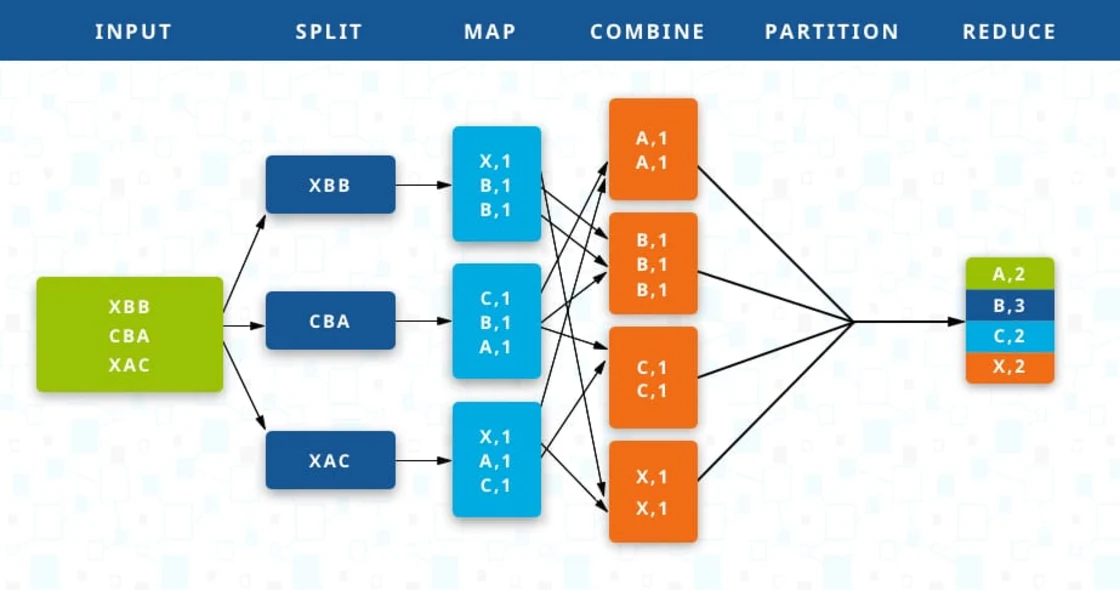
\includegraphics[scale=0.4]{mapreduce.jpg}
\newline
\newline
Hadoop wordt o.a. alleenstaand gebruikt tijdens de oefeningen Big Data, daarvoor kunnen we bestaande Docker Compose files gebruiken die de verschillende services bevatten nodig om een Master of Slave te starten.
In de eenvoudigste vorm is er 1 docker compose file die alle services opstart om te kunnen werken met 1 master en 1 slave.
\newline
\newline
Elke service (namenode, datanode, resourcemanager) is een specifiek Docker image, ook beschikbaar op DockerHub. Er zijn voorbeelden te vinden van de Docker scripts die gebruikt werden om dit soort images te bouwen. Typisch is er een basis Hadoop images dat het volledige framework bevat, en worden daar aparte images vanaf geleidt die telkens maar 1 specifiek process (namenode, datanode, ...) van Hadoop opstarten.
Door op die manier met aparte images te werken kan het beheer van de cluster buiten Hadoop worden gedaan, typisch in Kubernetes, zie verder.
\newline
\newline
In de volgende sectie gaan we Apache Spark bekijken, welke functionaliteit dit toevoegt aan Hadoop en hoe we dit kunnen integreren in Docker Compose.

\section{Spark}
Apache Spark is an open-source, distributed processing system used for big data workloads. It utilizes in-memory caching, and optimized query execution for fast analytic queries against data of any size.
Spark was designed for fast, interactive computation that runs in memory, enabling machine learning to run quickly. The algorithms include the ability to do classification, regression, clustering, collaborative filtering, and pattern mining.\autocite{AwsAmazon2023a}
\newline
\newline
Apache Spark is net als Hadoop een data processing engine voor big data. Spark verdeelt ook de taken en de gegevens over verschillende nodes, voor een aantal gevallen zal het sneller zijn dan Hadoop omdat het gebruik maakt van RAM geheugen in plaats van een bestandssysteem, dit is de Resilient Distributed Dataset (RDD).
\newline
\newline
Spark bevat meerder componenten om aan data verwerking te doen: Spark SQL, Spark MLlib en Spark GraphX.

\subsection{Spark SQL}
Spark SQL is a Spark module for structured data processing. It provides a programming abstraction called DataFrames and can also act as distributed SQL query engine. It enables unmodified Hadoop Hive queries to run up to 100x faster on existing deployments and data.\autocite{databricks2023}

\subsection{Spark MLlib}
Machine learning has quickly emerged as a critical piece in mining Big Data for actionable insights. Built on top of Spark, MLlib is a scalable machine learning library that delivers both high-quality algorithms (e.g., multiple iterations to increase accuracy) and blazing speed (up to 100x faster than MapReduce).\autocite{databricks2023}

\subsection{Spark GraphX}
Apache Spark's API for graphs and graph-parallel computation.
GraphX is a graph computation engine built on top of Spark that enables users to interactively build, transform and reason about graph structured data at scale. It comes complete with a library of common algorithms.\autocite{databricks2023}
\newline
\newline
Deze componenten kunnen in Hadoop MapReduce vervangen, en indien de datasets volledig in het cache geheugen passen, kan dan tot 100x sneller zijn.


\subsection{Spark Streaming}
Many applications need the ability to process and analyze not only batch data, but also streams of new data in real-time. Running on top of Spark, Spark Streaming enables powerful interactive and analytical applications across both streaming and historical data, while inheriting Spark’s ease of use and fault tolerance characteristics. It readily integrates with a wide variety of popular data sources, including HDFS, Flume, Kafka, and Twitter.\autocite{databricks2023}
\newline
\newline
Het is dit laatste onderdeel, Spark Streaming, dat door Kafka (zie verder) kan worden gebruikt om data aan door te geven voor verdere verwerking.
\newline
\newline
Terugkomend op ons doel van Spark in Docker containers te draaien, er zijn Spark Docker images beschikbaar die toelaten zowel een Spark Master als Worker te starten.
\newline
\newline
Er zijn ook voorbeelden te vinden van discussies over mogelijke manieren om Hadoop en Spark te combineren in Docker Compose.


\section{Kafka}
Apache Kafka is a distributed data store optimized for ingesting and processing streaming data in real-time. Streaming data is data that is continuously generated by thousands of data sources, which typically send the data records in simultaneously. A streaming platform needs to handle this constant influx of data, and process the data sequentially and incrementally.
\autocite{AwsAmazon2023b}

\subsection{Broker}
A Kafka broker receives messages from producers and stores them on disk keyed by unique offset. A Kafka broker allows consumers to fetch messages by topic, partition and offset. Kafka brokers can create a Kafka cluster by sharing information between each other directly or indirectly using Zookeeper.\autocite{GitBook2023}

\subsection{Topic}
What are Apache Kafka Topics? Apache Kafka has a dedicated and fundamental unit for Event or Message organization, called Topics. In other words, Kafka Topics are Virtual Groups or Logs that hold messages and events in a logical order, allowing users to send and receive data between Kafka Servers with ease.\autocite{Ishwarya2022}

\subsection{Partitions}
What Is a Kafka Partition? In Apache Kafka, partitions are the main method of concurrency for topics. A topic, a dedicated location for events or messages, will be broken into multiple partitions among one or more Kafka brokers\autocite{Carder2022}
\newline
\newline
Er zijn Kafka Docker images beschikbaar en er zijn ook voorbeelden te vinden van discussies over mogelijke manieren om Kafka en Spark te combineren in Docker Compose.
\newline
\newline
In vorige versies van Kafka werd Zookeeper gebruikt voor opslag van metadata. In recente versies is dit vervangen door een intern systeem, wat beter is omdat gebruikers dan geen extra applicatie moeten leren opzetten en er worden ook minder resources gebruikt.

\section{Zookeeper}
ZooKeeper is a centralized service for maintaining configuration information, naming, providing distributed synchronization, and providing group services. All of these kinds of services are used in some form or another by distributed applications. Each time they are implemented there is a lot of work that goes into fixing the bugs and race conditions that are inevitable.\autocite{ASF2023}
\newline
\newline 
What is ZooKeeper in Apache Kafka?
Zookeeper is used for metadata management in the Kafka world. For example: Zookeeper keeps track of which brokers are part of the Kafka cluster. Zookeeper is used by Kafka brokers to determine which broker is the leader of a given partition and topic and perform leader elections. \autocite{Conduktor2023}
\newline
\newline
Afhankelijk van de versie van Kafka die we uiteindelijk zullen gebruiken zal Zookeeper wel of niet toegevoegd worden aan de Docker compose.
\newline
\newline
\newline
\newline
\newline
Hadoop, Spark en Kafka worden al samen gebruikt volgens \textcite{Holmes2012}:
'In this situation, you'd use Kafka to both land data on Hadoop and provide a feed into a real-time data-streaming system such as Storm or Spark Streaming, which you could then use to perform near-real-time computations.' en \textcite{Leang2019}:
'one of the more significant findings to emerge from this study is that the integration of the Hadoop system especially Apache Kafka and Apache Spark enhances the performance and accuracy of data storing, processing, and securing in the manufacturing environment.'
\newline
\newline
Er is informatie te vinden over het gebruik van Docker compose om verschillende combinaties van 2 van de 3 frameworks te installeren maar niks over alle 3 samen, zeker niet met de requirements die wij willen onderzoeken (een afzonderlijke scalable beveiligde `cluster` per student).



\section{Virtual IT Company(VIC)}
VIC is een ``bedrijf'' in Hogent dat virtuele machines voorziet voor studenten, zodat bepaalde oplossingen niet op een eigen computer moet draaien, en op aanvraag maken ze de virtuele machine(s), er wordt een soort van contract afgesproken met machine specs en lifespan.
\newline
\newline
VIC gebruikt de oplossing van VMWare (vSphere, VMWare ESXi Hypervisor) voor het beheer van virtuele machines op de eigen hardware.

\subsection{Hypervisor}
A hypervisor, also known as a virtual machine monitor or VMM, is software that creates and runs virtual machines (VMs). A hypervisor allows one host computer to support multiple guest VMs by virtually sharing its resources, such as memory and processing.\autocite{VMware2023a}

\subsection{VMWare ESXi}
Discover a robust, bare-metal hypervisor that installs directly onto your physical server. With direct access to and control of underlying resources, VMware ESXi effectively partitions hardware to consolidate applications and cut costs. It’s the industry leader for efficient architecture, setting the standard for reliability, performance, and support.\autocite{VMware2023}

\subsection{vCenter}
vCenter Server is the centralized management utility for VMware, and is used to manage virtual machines, multiple ESXi hosts, and all dependent components from a single centralized location. VMware vMotion and svMotion require the use of vCenter and ESXi hosts.\autocite{Abbas2023}
\newline
\newline
Momenteel wordt er nog geen Kubernetes gebruikt in het VIC. Ook geen Docker containers, alles is gebaseerd op virtuele machines.
\newline
\newline
VMWare vSphere, dit is de set van VMWare Virtualization applicaties, ondersteunt intussen ook Kubernetes.
\newline
\newline
De volgende componenten zijn van belang om het gebruik van Kubernetes op VMware te begrijpen. De concepten van Kubernetes worden gelinkt aan VMWare concepten.

\subsection{Nodes}
There are two main node types in Kubernetes, a Master and Worker. A master node is a management node, what you would expect of vCenter Server. A worker node is what you would expect of an ESXi host, allowing you to run Pods.\autocite{VMware2019}

\subsection{Pod}
A Pod is a group of one or more containers. If we map this to a VMware Administrator construct think of Pods as an object similar to a virtual machine. Pods are managed by the Kubelet that runs on each node. Kubelet watches Podspecs assigned to it and handles all lifecycle by comparing actual Pod state to the desired state stored in the Podspec.\autocite{VMware2019}

\subsection{Namespace}
A Namespace is used as the unit of management in environments with many users across multiple teams or projects. Namespaces are a way to divide cluster resources and separate permissions between users. When a Namespace is created you assign CPU, Memory and Storage limits to restrict the amount of resources a workload can consume, not unlike a vSphere Resource Pool. Where Namespaces differ from Resource Pools is that they also incorporate controls such as security. For example, from a security perspective via Namespaces you can manage access controls by using edit or read-only groups. You also have the ability through security policies to limit ports, audit changes and force encryption of data. To encrypt all containers and/or VMs in a Namespace is done by setting one property rather than going to each VM and encrypting individually.\autocite{VMware2019}
\newline
\newline
Kubernetes wordt ondersteund om Developers te laten werken met gekende tools en begrippen zodat ze zich niet moeten verdiepen in VNWare vSphere.
\newline
\newline
To a developer, vSphere with Kubernetes looks and acts like a standard Kubernetes cluster. Their tools and processes work across implementations. They can use the Kubernetes “declarative syntax” to define what resources they need, such as storage, networking, and even relationships \& availability requirements. By using the industry-standard Kubernetes syntax they don’t need direct access to, or knowledge of, the vSphere APIs, clients, or infrastructure.\autocite{VMware2019}
\newline
\newline
Daarnaast worden Docker containers en Docker Compose ondersteund door VNWare vSphere, dus dit is ook nog een mogelijke oplossing zonder Kubernetes. 
\newline
\newline
\newline
Om te onderzoeken hoe aan de security en stability (isolatie van gebruikers) eisen kan worden voldaan, gaan we o.a. Namespaces verder bestuderen. Daarnaast gaan we ook bekijken in hoeverre het gebruik van een reverse proxy (bv. Nginx) de toegang tot een Pod kan afschermen om op die manier maar 1 student per Pod toe te laten te connecteren op de consoles van Hadoop, Spark en Kafka.
\newline
\newline
Voor de configuratie van Nginx basic authentication en users kijken we o.a. naar Kubernetes ConfigMap.

\subsection{ConfigMap}
A ConfigMap is an API object used to store non-confidential data in key-value pairs. Pods can consume ConfigMaps as environment variables, command-line arguments, or as configuration files in a volume.
A ConfigMap allows you to decouple environment-specific configuration from your container images, so that your applications are easily portable.\autocite{Kubernetes2023}

%%=============================================================================
%% Methodologie
%%=============================================================================

\chapter{\IfLanguageName{dutch}{Methodologie}{Methodology}}%
\label{ch:methodologie}



%% TODO: Hoe ben je te werk gegaan? Verdeel je onderzoek in grote fasen, en
%% licht in elke fase toe welke stappen je gevolgd hebt. Verantwoord waarom je
%% op deze manier te werk gegaan bent. Je moet kunnen aantonen dat je de best
%% mogelijke manier toegepast hebt om een antwoord te vinden op de
%% onderzoeksvraag.

Uit de studie van alle betrokken onderdelen, zijnde Containertechnologie, Big Data en VIC infrastructuur in vorig hoofdstuk lijkt het dat een installatie gebaseerd op containers op veel manieren kan. In dit eerste deel gaan we dieper in op die verschillende mogelijkheden.

\section{Welke oplossingen zijn mogelijk?}

Bij elk platform is het de bedoeling de gebruikers een aangename ervaring te bieden, daarbij is performantie een belangrijk onderdeel, vooral bij Big Data oplossingen waar het verwerken van grote volumes data veel tijd kost en soms in bijna real-time dient te gebeuren.
In het streven naar goede performantie speelt schaalbaarheid een belangrijke rol, en de architectuur van Hadoop, Spark en Kafka ondersteunt volop het inschakelen van extra ``machines'' bij een toenemend aantal gebruikers en behoefte aan meer snelheid en verwerkingscapaciteit.
Bij een typische installatie van deze oplossingen zou een cluster van elke oplossing apart opgezet worden. Elke cluster kan dan onafhankelijk op- en neerschalen naargelang de nood.
\newline
De schaalbaarheid bij Spark bijvoorbeeld, is doordat het werk verdeeld wordt over meerdere Executors en er dus in een cluster eenvoudig extra Executors kunnen gebruikt worden. Zie ook volgende figuur.
\newline
\begin{figure}
    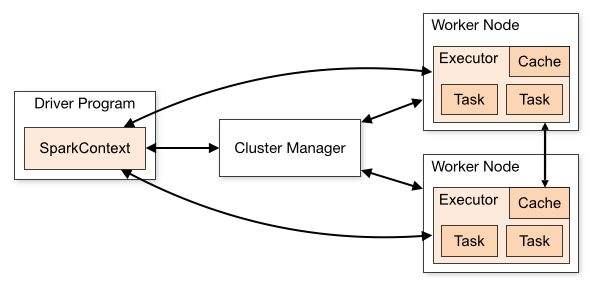
\includegraphics[scale=0.7]{cluster-overview.png}
    \caption{TODO \autocite{Spark2023e}}
\end{figure}

Een van de onderdelen van Hadoop is YARN, een resource manager en job scheduler die instaat voor de verdeling van het werk over de verschillende cluster nodes en dus zorgt voor de schaalbaarheid.
\newline
\begin{figure}
    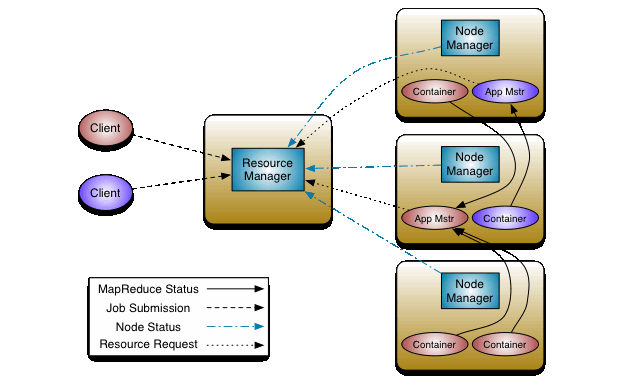
\includegraphics[scale=0.7]{yarn_architecture.png}
    \caption{TODO \autocite{Hadoop2023d}}
\end{figure}

Merk op dat het bij real-world installaties van deze applicaties, het meestal de bedoeling is dat de Big Data oplossingen achterliggend gebruikt worden door eigen applicaties en dat gewone ``gebruikers'' op geen enkele manier rechtstreeks toegang krijgen tot bv. Hadoop of Spark.
\newline
Volgens \autocite{Hadoop2023} wordt in een standaard configuratie de Hadoop cluster eenvoudig beschermd door alle netwerk toegang te beperken. 
Bij de meeste installaties zou dit volstaan als beveiliging, en krijgen enkel de gekende applicaties die er gebruik van maken de netwerk toegang tot de Big Data oplossingen.
\newline
\newline
Dit is niet het geval voor ons, de bedoeling is juist dat de studenten rechtstreeks gebruikmaken van de oplossingen, waarbij één van de doelstellingen van deze bachelorproef is om de verschillende gebruikers (studenten), zowel tijdens de les als tijdens examens volledig afgezonderd te laten werken. Die afzondering geldt zowel op gebied van security als stabiliteit.

\subsection{Security}

\subsubsection{Hadoop Secure mode}
Volgens \textcite{Kiran2022} biedt Hadoop security alle onderdelen van een typische beveiliging: authenticatie, authorisatie, auditing en encryptie van data.
De authenticatie steunt op Kerberos, volgens \textcite{Kerberos2023} een netwerk authenticatie protocol gebaseerd op encryptie en geheime sleutels. Het wordt typisch gebruikt in omgevingen met meerdere partijen die elkaar moeten vertrouwen en waarvoor dus authenticatie vereist is. Er is een implementatie beschikbaar, gemaakt door het MIT en het is beschikbaar zowel als Docker Image als in de typische Linux distributies.
\newline
Volgens \textcite{Hadoop2023} is een zeer goede kennis van Kerberos en DNS vereist om Hadoop services op te zetten in 'secure mode'.
\newline
\newline

\subsubsection{Secure HDFS}
Volgens \textcite{Hadoop2023b} ondersteunt HDFS het gebruik van READ, WRITE en EXECUTE permissies. Daartoe worden alle bestanden en folders geassocieerd met één gebruiker, de eigenaar genoemd, en één groep van gebruikers.
Op die manier kunnen dan permissies toegekend worden aan de eigenaar, aan de groep en aan alle gebruikers. Dit is typisch ook de manier waarop permissies in Linux systemen functioneren.
\newline
Voor gebruikers van Linux komt ook de syntax voor het beheer van de permissies komt bekend voor:
TODO
hdfs dfs –chmod -R go+w <file/dir>


Voorwaarde voor de toepassing van deze permissies is dat de gebruiker is gekend, geauthentificeerd door Kerberos, en dat de groepen waartoe de gebruiker behoort gekend zijn. Voor dit laatste doet HDFS volgens \textcite{Hadoop2023c} een beroep op bijvoorbeeld het Operating Systeem of een LDAP server.


\subsubsection {Spark authenticatie en authorisatie} \autocite{Spark2023c}
Net zoals bij Hadoop zijn security functionaliteiten zoals authenticatie niet actief bij een standaard installatie van Spark. Als er geen afscherming is van de netwerk toegang, moet communicatie tussen de Spark processen afgeschermd worden d.m.v. authenticatie en encryptie, en moet voor de lokale opslag ook encryptie gebruikt worden. De Web User Interface moet beschermd worden door authenticatie, en daarvoor moeten Java servlet filters gebruikt worden, die echter niet door Spark worden aangeboden en dus moeten gebouwd worden op maat van het systeem dat de authenticatie zal doen.
Er zijn voorbeelden te vinden van dit soort filters, meestal gebaseerd op Basic Authentication (zie verder bij nginx). Op volgende blog vind je een voorbeeld van een eigen gebouwde filter die een login pagina toevoegt aan Spark: \textcite{Cacoveanu2019}
\newline
\newline


\subsubsection{Apache Sentry, Apache Ranger, Apache Knox}
Het evolueert allemaal zeer snel in het Hadoop ecosysteem. Volgens \textcite{Chu2020}, een artikel uit 2020 over Hadoop Security, is Apache Sentry de populaire tool voor Authorizatie. Maar kort daarna werd Apache Sentry een verlaten project en is het verhuisd naar de Attic.
\newline
Volgens \textcite{Anand2021} is dit het gevolg van het samengaan van 2 platformen waarbij de keuze is gemaakt om Sentry te vervangen door Ranger. Het artikel bevat een gedetailleerde vergelijking tussen de functionaliteiten van beide oplossingen.
\newline
In https://ysoo23.medium.com/discussion-and-comparison-of-several-hadoop-security-tools-b4532a8c67f9 is er een vergelijking met nog andere tools en daaruit komt Apache Ranger als de beste keuze.


\subsubsection {Kafka}
Volgens \textcite{Maarek2018} ondersteunt Kafka meerdere beveiligingsmechanismes zijnde:
\begin{itemize}
    \item Encryptie van alle data die tussen de Producers, Kafka en de Consumers wordt uitgewisseld. Dit is in ons geval van geen belang, we willen vooral de toegang van de studenten tot elkaars werk afschermen, we gaan er niet van uit dat de gegevens die op het netwerk worden uitgewisseld kwetsbaar zijn gedurende de beperkte periode van een les of examen.
    \item Authenticatie met SSL of SASL: de toegang tot de Kafka cluster wordt enkel toegelaten voor gebruikers die zich kunnen identificeren. Deze identificatie kan met ``SSL'', waarbij de Kafka broker de identititeit van de applicatie verifieerd door middel van SSL certificaten, of met een aantal andere authenticatie mechanismes gaande van PLAINTEXT (eenvoudige gebruikersnaam/paswoord combinatie) tot GSSAPI (Kerberos tickets). Merk op dat ook in deze gevallen SSL wordt gebruikt om op een veilige manier te communiceren.
    \item Authorizatie laat toe om de permissies te definiëren die bepalen of een bepaalde geïdentificeerde gebruiker (applicatie) toegang krijgt tot bepaalde topics om te lezen of the schrijven.
\end{itemize}

Gebruikers afschermen van elkaar in een opstelling van Hadoop en Spark, beiden in clusters wordt snel zeer ingewikkeld. Elk van de oplossingen bestaat uit meerdere processen die met elkaar communiceren en ieder onderdeel moet secure opgezet worden zodat gebruikers niet, bewust of per ongeluk, data van elkaar te zien krijgen. We spreken hier over encryptie voor de opslag, authenticatie en encryptie bij communicatie tussen de verschillende processen, authenticatie voor de gebruiker op Hadoop, authenticatie voor de gebruiker op Spark enz.
De manier van beveiligen is voor elk van deze oplossingen en interne processen op een andere manier, en vraagt om bijkomende softwares zoals LDAP, Kerberos server, enz.

Voor Kafka is de SASL/PLAINTEXT beveiliging zeker voldoende in ons geval en ook relatief eenvoudig op te zetten. Dit gaan we verder dan ook uitproberen.

\subsection{Stabiliteit}
Elk van de Big Data oplossingen, en Kubernetes, ondersteunen mechanismes om applicaties te verdelen over de pods en van elkaar af te schermen, bij bepaalde onderdelen kunnen er limieten gezet worden op CPU en geheugen gebruik. Deze configuraties zijn gekoppeld aan nodes, containers en applicaties. De achterliggende bedoeling is vooral om de eigen gebouwde applicaties te ondersteunen en vlot te laten beroep doen op de Big Data functionaliteiten. De focus van deze mechanismes, dikwijls gebaseerd op een voorkennis van het soort verwerken dat in de cluster zal gebeuren, ligt minder op rechtstreeks gebruik van de oplossingen door gebruikers die applicaties aan het ontwikkelen zijn.
\newline
\newline
In \textcite{Deane2019} wordt hier dieper op ingegaan en wordt gesproken over het ``lawaaierige buurman probleem''. Het legt uit dat hoe meer gebruikers er komen in de cluster, hoe moeilijker het wordt om ervoor te zorgen dat deze gebruikers geen last van elkaar ondervinden. Daartoe passen beheerders allerlei technieken toe zoals YARN resource pools, prioriteiten stellen, specifieke nodes toewijzen aan applicaties, enz. Een aantal van deze technieken zijn ook niet toepasbaar in ons geval want alle ontwikkelaars moeten gelijk behandeld worden, dus prioriteiten zetten is niet haalbaar, en specifiek werk opslitsen op specifieke nodes is ook niet mogelijk tenzij dan door alle ontwikkelaars aparte nodes te geven.
De oplossing die volgens https://blog.cloudera.com/improving-multi-tenancy-with-virtual-private-clusters/ dan typisch gebeurt is opslitsen van de cluster in kleinere clusters. Gezien het hier meestal gaat over dezelfde data van een bedrijf bevat elke cluster dan een duplicaat en hierop gaat het artikel dan verder en stelt een soort tussenmodel voor, waarbij de HDFS data op een gedeelde cluster blijft en de MapReduce en Spark verwerking op aparte clusters gebeurt.
\newline
Aangezien het in ons geval gaat om het gebruik van de cluster door minder ervaren ontwikkelaars, is de kans op ``lawaaierige buren'' groot.


\subsection{Installatie met containertechnologie}
In vorig hoofdstuk kwam de containertechnologie uitgebreid aan bod en gebaseerd op alle informatie die we onderzochten lijkt het gebruik van containers een goede piste om de installatie te vereenvoudigen.
\newline
We zagen ook dat er meerdere mogelijkheden zijn om zo'n installatie op te zetten, zoals Kubernetes, Docker Swarm, Docker Compose, Docker.
\newline
Bij elk van de gebruikte applicaties moeten dus een aanzienlijk aantal nodes opgezet worden voor een basis cluster, gedefinieerd, geconfigureerd en geïnstalleerd.
\newline
De configuratie kan bijvoorbeeld geconfigureerd worden via Kubernetes of Docker Swarm, gedefinieerd in YARN die dan beroep doet op Docker om extra containers te starten. Of volgens \textcite{Spark2023d}, Spark die rechtstreeks kan gebruikmaken van Kubernetes, om Executors op Kubernetes Pods aan te maken en er applicaties op uit te voeren.
\newline
\newline

\subsection{Conclusie}
De eerste vraag die we hier proberen te beantwoorden is of een gedeelde cluster de beste oplossing is voor de oefeningen en het examen van de cursus Big Data. Het alternatief is een aparte omgeving voor elke student.
\newline
De installatie van zowel de gedeelde cluster als de aparte omgeving kan geautomatiseerd worden met voornoemde containertechnologie.
\newline
We zien een aantal mogelijke redenen om te kiezen voor een gedeelde Big Data cluster: reden 1 is gedeelde data, reden 2 is optimaal gebruik van resources en reden 3 is de enkelvoudige installatie t.o.v. een installatie voor elke student.

\subsubsection{Gedeelde data}
Dit is hier niet van toepassing, de data is enerzijds niet van die omvang dat ze niet kan gedupliceerd worden voor elke student en daarnaast is het ook niet de bedoeling dat de studenten dezelfde data kunnen wijzigen.

\subsubsection{Optimaal gebruik van resources}
Hét argument voor optimaal gebruik van resources is dat nodes in een cluster gedeeld worden door alle gebruikers en ter beschikking staan voor het uitvoeren van bewerkingen naargelang de vraag, die niet doorlopend dezelfde is. Op die manier kan aan de afwisselende vraag van de gebruikers worden voldaan door een beperkter aantal nodes dan indien ze vastgelegd zouden zijn per applicatie, en dus gedurende bepaalde ongebruikt zijn.
\newline
In het geval van de studenten is dit niet van toepassing want juist tijdens de oefeningen en het examen wordt er op intensieve manier gebruikt gemaakt van de Big Data cluster en zal een gedeelde cluster voortdurend op piekvermogen moeten draaien.
\newline
Merk op dat het wel waarschijnlijk is dat de installatie van één enkele gedeelde cluster minder resources zal gebruiken dan de aparte omgevingen per student.

\subsubsection{Enkelvoudige installatie}
Het achterliggende idee van gebruik van containertechnologie is dat het eenvoudig is om een container op te starten, te verplaatsen, bijkomende containers te starten, enz. Dit alles gebaseerd op een set Docker images in combinatie met configuratie files.
\newline
Het werk kruipt dus eerder in dit alles opzetten, en is grotendeels onafhankelijk van hoeveel keer het daarna geïnstalleerd moet worden.
Een gedeelde cluster zal complexer zijn om op te zetten door de security en stabiliteitsvereisten.
\newline
Zoals ook aangehaald in het vorige stuk over stabiliteit, zal er altijd het risico blijven dat de studenten niet 100\% afgeschermd zijn van elkaar en van onbetrouwbare applicaties.
\newline
Gebaseerd op het voorgaande lijkt het ons dus beter, en eenvoudiger, is om elke student een eigen omgeving te geven, volledig afgeschermd van de andere, door aparte containers te gebruiken per student.
\newline
De nodige combinaties van containers, nodig voor de oefeningen of het examen, kunnen we opzetten door gebruik te maken van Docker Compose of Kubernetes files die een specifieke combinatie definiëren van de Big Data oplossingen. Voor elke student wordt dan naargelang de les de specifieke omgeving opgestart.
\newline
Merk op dat de Kubernetes of Docker Compose configuratie files die we verder in dit hoofdstuk gaan opbouwen het startpunt zijn voor elk van deze omgevingen, maar niet voldoende. De basis dient aangepast/uitgebreid te worden met specifieke configuraties gerelateerd aan de omgeving, zoals definitie van netwerken en adressen, volumes, enz. Dit dient nog verder uitgewerkt te worden, naargelang de uiteindelijke keuzen van Container Cluster oplossing, om tot een finale oplossing te komen.
\newline
Dit kan uiteindelijk allemaal geautomatiseerd worden maar betekent dat de docent toegang moet hebben tot Kubernetes, Docker Swarm of een VIC UI omgeving om het uit te voeren.
\newline
Een bijkomend voordeel van dit soort aanpak, elke student een eigen omgeving, is dat ze niet alleen kan gebruikt worden om applicaties op de Big Data oplossingen te ontwikkelen, maar ook om studenten de administratie van de Big Data oplossingen zelf op hun eigen geïsoleerde omgeving te leren. Al is dat vandaag niet de focus van de lessen, op hun eigen omgeving kunnen ze Admin zijn zonder impact op anderen.
\newline
\newline


\section{Big data}

Om meer vertrouwd te geraken met de Big Data oplossingen zijn deze eerst allemaal eens lokaal opgezet via Docker Compose configuraties. Zie Appendix [B: Docker compose].
Daarbij is er vertrokken van voorbeelden die beschikbaar zijn op het Internet en voorbeelden uit de Big Data cursusoefeningen.
\newline
\newline
Dit verliep vlot. Pas tijdens het omzetten naar Kubernetes, zie verder, bleek dat het gebruik van Docker en Docker Compose lokaal voor heel wat voordelen zorgt. Bijvoorbeeld dat je eenvoudig een shell kunt openen in om het even welke lokale Docker container en daar commandos kunt uitvoeren die gebruik maken van de geïnstalleerde software in die container. Dit wordt voor de oefeningen gebruikt om bijvoorbeeld Hadoop commandos uit te voeren terwijl er op de lokale machine geen hadoop beschikbaar is. Via 'docker exec' kan de student op de lokale Namenode container aanloggen, er files naar kopiëren en die dan via 'hadoop' commandos naar hdfs in de andere container overbrengen, of Java programma's opstarten.
Eens de lokale omgeving naar de cloud verhuisd zal zijn kan dit niet meer gebruikt worden en moet hiervoor een andere oplossing komen.` Dit gaan we later opnemen en dieper bespreken.'

\section{Security}
We gaan dus niet voor een volledige, alle producten, alle processen, alle communicatie, secure installatie want 1 enkele omgeving voor 1 student zal volledig binnen 1 Pod draaien en in eerste instantie dus ook volledig afgeschermd zijn.
De uitdaging is nu eerder om bepaalde poorten toegankelijk te maken om toe te laten met deze omgeving te werken, maar we willen de toegang tot deze poorten voor elke omgeving wel beperken tot 1 student.

\subsection{Apache Knox}
Zoals eerder al aangehaald is Apache Knox een security oplossing die toe laat een Hadoop cluster af te schermen.
Volgens (https://knox.apache.org/) is het een gateway die de toegang tot de cluster vormt voor alle interacties (REST en HTTP), en die authenticatie doet van de gebruikers. Voor die authenticatie worden de typische protocols ondersteunt zoals LDAP/ActiveDirectory, Kerberos, SAML en OAuth. Dit is ideaal in een onderneming om bestaande gebruikers toe te laten, maar voelt overdreven (overkill) in ons geval van 1 gebruiker per omgeving. Er moest dus naar iets eenvoudigers gezocht worden.

\subsection{Kubernetes services}
Services in Kubernetes zijn een manier om toegang te verlenen tot de netwerk applicaties die in één of meerdere Pods in de cluster draaien. Aangezien deze applicaties op elk moment van Pod kunnen wijzigen of in meerdere Pods opgestart worden, is er een mechanisme nodig die dit opvangt en zorgt dat de applicaties toegankelijk blijven voor de buitenwereld. Dit zijn de Kubernetes Services.
\autocite{Kubernetes2023b}

Er zijn meerdere types services maar voor onze oplossing is het Ingress type van belang omdat het gewoon een HTTP(S) ingangspunt is in combinatie met regels voor routing. Achterliggend is 1 van de implementaties de Ingress-Nginx controller. Dit is een integratie van Nginx uitgebreid met Kubernetes integratie mechanismes voor o.a. herstarten/herladen bij configuratie wijzigingen. Bij onze opzet zijn er geen wijzigingen eens de omgeving is opgestart, dus heb werd er een test opgezet met een gewone Nginx die dan deel uitmaakt van de Kubernetes Pod.
\autocite{Kubernetes2023d}


\subsection{Nginx}
Nginx (https://www.nginx.com/) is een web server die dikwijls als ingangspunt van een web site gebruikt wordt (Reverse proxy TODO \autocite{Wikipedia2023d}) en die zorgt dat de achterliggende structuur afgeschermd is voor de buitenwereld. Daarnaast kan het zorgen voor Load Balancing TODO \autocite{Wikipedia2023c} en beveiliging (HTTP Basic Authentication, SSL/TLS offloading).
\newline
\newline


\subsubsection{HTTP Basic Authentication}
TODO \autocite{Wikipedia2023b}
Basic Authentication is een optioneel onderdeel van een HTTP(S) transactie waarbij aan de initiërende partij, typisch de webbrowser, gevraagd wordt een gebruikersnaam en paswoord te verstrekken. Het is de eenvoudigste techniek voor het afdwingen van toegangscontroles tot web resources, omdat hiervoor geen cookies, sessie-ID's of inlogpagina's nodig zijn.
Omdat de inloggegevens in de header van elk HTTP(S)-verzoek moeten worden verzonden, moet de webbrowser ze gedurende een redelijke tijd in de cache opslaan om te voorkomen dat de gebruiker voortdurend om zijn gebruikersnaam en wachtwoord wordt gevraagd.
Merk op dat de inloggegevens die verstuurd worden (gebruikersnaam en paswoord) niet beschermd zijn, ze zijn gecodeerd met base64 encoding maar dit biedt geen enkele bescherming. Daarom wordt Basic Authentication meestal gebruikt in combinatie met HTTPS om vertrouwelijkheid te bieden. Aangezien het in onze oplossing over tijdelijke omgevingen gaat is het gevaar dat bij HTTP de inloggegevens onderschept worden minimaal en kan dit dus ook voor niet-HTTPS gebruikt worden.
\newline
\newline
Basic Authentication lijkt me voldoende, per omgeving moeten dan de inloggegevens voor 1 gebruiker, de student, opgezet worden. Nginx ondersteunt meerdere mechanismen voor authenticatie waaronder een eenvoudig paswoord bestand. Deze is in het formaat
\newline
\newline
\begin{lstlisting}
user1:$apr1$/woC1jnP$KAh0SsVn5qeSMjTtn0E9Q0
user2:$apr1$QdR8fNLT$vbCEEzDj7LyqCMyNpSoBh/
user3:$apr1$Mr5A0e.U$0j39Hp5FfxRkneklXaMrr/ 
\end{lstlisting}


en wordt gegenereerd door Linux tools zoals htpasswd (deel van apache2-utils en httpd-tools), waarbij het paswoord van een gebruiker met MD5 wordt geëncrypteerd. In ons geval zou dit bestand dus de unieke student gebruiker bevatten, met verschillend paswoord per omgeving.
Optioneel kan overal een extra account voor de lesgever, met identiek paswoord voor alle omgevingen, toegevoegd worden.
\newline
\newline
Als eerste onderzoek voor dit security onderdeel is er, om de configuratie van de Basic Authenticatie te bouwen, een beperkte Kubernetes yaml file gemaakt met alleen maar nginx, deze start en stopt snel tijdens het testen, maar liet al direct toe om Kubernetes Services, Port mapping en Configmap te gebruiken. Dit was ook de eerste keer dat Kubernetes werd gebruikt en dus lokaal moest geïnstalleerd worden.
\newline
\newline
\subsubsection{Configmaps} 
\autocite{Kubernetes2023}
\newline
Een ConfigMap wordt gebruikt om niet-beveiligde configuratie gegevens te beheren in sleutel-waarde formaat, en ter beschikking te stellen van de Pods en Containers, als omgevingsvariabele of als (configuratie) bestand via een volume.
Een ConfigMap bevat typisch de configuratie die is losgekoppeld van het Docker image om op die manier images meer generiek inzetbaar te maken.\textcite{Kubernetes2023}


Initieel waren er hier problemen met het configureren van de volumes omdat Kubernetes volumes op een andere manier werken dan de volumes van Docker Compose, waar er eenvoudig verwezen kan worden naar lokale folders op de machine waar de container draait, terwijl bij Kubernetes alles in de Configmap gestopt wordt om op die manier van Pod te kunnen switchen of uitbreiden, en de configuratie (files) mee moet kunnen naar alle pods.
\newline
\newline
In de ConfigMap werd de nginx.conf file gestopt en de paswoord file voor Basic Authentication.
Uiteindelijk met volgende configuratie kwam de popup voor Basic Authentication te voorschijn.
\newpage
\begin{lstlisting}
user  nginx;
worker_processes  1;

error_log  /var/log/nginx/error.log warn;
pid        /var/run/nginx.pid;

events {
    worker_connections  1024;
}
http {
    include       /etc/nginx/mime.types;
    
    default_type  application/octet-stream;
    
    log_format  main  '$remote_addr - $remote_user [$time_local] "$request" '
    '$status $body_bytes_sent "$http_referer" '
    '"$http_user_agent" "$http_x_forwarded_for"';
    
    access_log  /var/log/nginx/access.log  main;
    
    sendfile        on;
    
    keepalive_timeout  65;
    
    server {
        listen 443 ssl;
        listen [::]:443 ssl;
        
        server_name         www.hadoop.local;
        ssl_certificate     /etc/nginx/ssl/tls.crt;
        ssl_certificate_key /etc/nginx/ssl/tls.key;
        ssl_protocols       TLSv1 TLSv1.1 TLSv1.2;
        ssl_ciphers         HIGH:!aNULL:!MD5;
        
        proxy_set_header Host $host;
        proxy_set_header X-Forwarded-For $proxy_add_x_forwarded_for;
        
        proxy_cache_revalidate on;
        proxy_cache_use_stale error timeout http_500 http_502 http_503 http_504;
        proxy_cache_background_update on;
        proxy_cache_lock on;
        
        resolver kube-dns.kube-system.svc.cluster.local valid=5s;
        
        auth_basic "Access restricted";
        auth_basic_user_file /etc/nginx/password.conf;
        
        location / {
            root /usr/share/nginx/html;
            index index.html index.htm;
        }
    }
}
\end{lstlisting}

[TODO] - Eigen Docker image voor nginx docker + config via ENV
Hier is nog een idee om verder te automatiseren door aan de Nginx Docker container de gebruikersnaam en paswoord te geven en die gaat dan intern htpasswd gebruiken om de Auth file te genereren. Nog verder uit te werken ?
https://github.com/dtan4/nginx-basic-auth-proxy
\newline
\newline
\begin{lstlisting}
version: '2'
services:
web:
image: tutum/hello-world:latest
nginx:
image: quay.io/dtan4/nginx-basic-auth-proxy:latest
ports:
- 8080:80
- 8090:8090
environment:
- BASIC_AUTH_USERNAME=username
- BASIC_AUTH_PASSWORD=password
- PROXY_PASS=http://web/
- PROXY-SERVERNAME=hadoop.student1.hogent.be

\end{lstlisting}

\section{Hadoop}
Daarna werd Hadoop toegevoegd en de configuratie voor nginx om als Reverse Proxy gebruikt te worden voor Hadoop. Hierbij is vertrokken van de Docker Compose file die was opgebouwd en getest in vorige stappen, en heb die toegevoegd aan de Kubernetes file maar bij het opstarten waren er een aantal problemen. De namenode was niet bereikbaar voor de datanode, resourcemanager en historyserver.
In een Docker compose file worden alle containers verbonden via 1 of meerdere virtuele netwerken, en zorgt Docker ervoor dat de containers naar elkaar kunnen verwijzen door middel van de containernaam. Dit is niet het geval bij Kubernetes (of vSphere), waar de naam van de Pod, waarop de container draait, moet worden gebruikt. Aangezien in onze oplossing alle containers voor 1 student op dezelfde Pod draaien kunnen we ook 'localhost' gebruiken.\newline
In de configuratie voor Kubernetes moest dus bij elke container de verwijzing naar andere containers (hostnamen) vervangen worden door 'localhost'.
\newline
\newline
Om de configuratie van Hadoop aan te passen zijn er 2 manieren, ofwel gebruikmakende van environment variabelen gedefinieerd rechtstreeks op de container ofwel met environment variabelen gedefinieerd in een aparte ConfigMap. Typisch worden beiden gebruikt, in de ConfigMap stoppen we variabelen die voor alles containers gelijk zijn, op de container de variabelen die verschillend zijn per container. Een voorbeeld van de laatste soort is SERVICE\_PRECONDITION die een manier is om de bepalen op welke andere containers moet gewacht worden. Dit is een mechanisme van Apache, waarbij een specifieke applicatie wacht met opstarten tot het contact krijgt met die andere applicatie.
\newline
\newline
Na deze aanpassingen leek het nog niet voldoende om alles werkend te krijgen maar uiteindelijk bleek het te liggen aan de ConfigMap die ook nog elementen van nginx bevatte.
\newline
\newline
Eens Hadoop werkende in Kubernetes, werd de reverse proxy configuratie van nginx aangepakt. Eerst door een Hadoop context toe te voegen aan de URL, bv http://localhost/hadoop, en die dan via de nginx proxy\_pass door te sturen naar Hadoop.
\newline
\newline
\begin{lstlisting}
location / {
    proxy_set_header Host $http_host;
    proxy_redirect off;
    # rewrite ^/hadoop/(.*)$ /$1 break;
    proxy_pass http://localhost:9870/;
}

\end{lstlisting}

Daarbij trad volgend probleem op:
\newline
\newline
- Browser vraagt http://localhost/hadoop
- Browser krijgt HTML terug van Hadoop, via nginx
- HTML bevat verwijzingen naar /static/bootstrap.css
\newline
\newline
Een mogelijke oplossing hiervoor is ofwel nginx de HTML te laten aanpassen (filteren) en regels te definiëren die overal '/hadoop' toevoegen aan links van images, css, enz. Hierbij is er een kans dat we niet alle gevallen vinden en toevoegen aan de filter.
Een andere oplossing is om een apart DNS adres (servernaam) te gebruiken voor Hadoop, nginx kan dan op basis van de servernaam de requests doorsturen naar Hadoop. Hiervoor moest lokaal de hosts file van Windows 
\newline
(C:/Windows/System32/drivers/etc) gewijzigd worden en het volgende toegevoegd:
127.0.0.1 www.hadoop.local
\newline
\newline
De reverse proxy configuratie moest ook aangepast worden omdat het niet langer op url (location /hadoop) werkt maar op servernaam.
\newline
\newline
\begin{lstlisting}
server {
    listen 80;
    listen [::]:80;
    server_name localhost;
}

\end{lstlisting}

Bij surfen in de browser naar http://www.hadoop.local, kwam er nu eerst de user/paswoord popup en pas na invullen van de correcte gegevens kwam de WebUI van Hadoop.

\section{HTTPS/SSL}

Om de installatie veiliger te maken is er beslist om HTTPS op te zetten. Het is voldoende om dit op nginx te configureren want dat is de enige server en communicatie die van buitenaf zichtbaar is en dus mogelijk kan bespioneerd worden. Er zijn nog een aantal voordelen dat dit enkel op de nginx server moet gebeuren:
\newline
\newline
- Performantie: SSL maakt zwaar gebruik van de CPU en op deze manier worden de andere containers hiermee niet belast.
- Certificaat beheer: installatie en onderhoud van de certificaten moet maar op 1 plaats gebeuren
- SSL software patching: indien kwetsbaarheden ontdekt worden in de SSL software moet de installatie van security patches enkel op de nginx gebeuren, eenvoudig door naar een nieuw image te verwijzen.
\newline
\newline
Het opzetten van SLL op een aparte server, nginx in dit geval noemt men 'SSL offloading'.

\subsection{Certificaat}

Om SSL op te zetten bij nginx is een certificaat nodig. Voor de lokale testen werd er een certificaat gegenereerd gebruikt makende van openssl. Aangezien dit niet standaard al op Windows geïnstalleerd is, is er een tijdelijke Docker image gebruikt: alpine/openssl.
\newline
\newline
Met volgende commando kon werd een certificaat aangemaakt dat vanuit de Docker container bewaard werd op de laptop.
\newline
\newline

docker run -ti --rm -v \$(pwd):/apps -w /apps alpine/openssl <openssl\_command>

\begin{lstlisting}
server {
    listen              443 ssl;
    server_name         www.hadoop.local;
    ssl_certificate     /etc/nginx/ssl/tls.crt;
    ssl_certificate_key /etc/nginx/ssl/tls.key;
    
    location / {
        proxy_pass ...
    }
}
\end{lstlisting}

\section{Spark}

De volgende stap was een Kubernetes yaml bestand voor de combinatie Nginx, Hadoop en Spark. Dit verliep vlot, dezelfde problemen als bij Hadoop, vooral docker container namen die omgezet moesten worden naar localhost, enz die we intussen al snel herkenden.
\newline
\newline
Docker Compose biedt een functionaliteit die in Kubernetes niet bestaat, namelijk 'depends\_on'. Deze laat toe om de afhankelijkheid van containers te definiëren zodat containers niet starten voordat andere nodige containers zijn gestart. Dit wordt gebruikt bij Spark worker die (depends\_on) Spark master nodig heeft.
Bij Hadoop wordt dit opgelost door een eigen aanpak, de SERVICE\_PRECONDITION (zie eerder vermeld bij Hadoop).
\newline
\newline
Spark heeft daar geen oplossing voor maar uiteindelijk bleek dat de Spark processen hier geen hinder van ondervonden en dus het gebrek aan de 'depends\_on' geen probleem vormt.
\newline
\newline
Net zoals bij Hadoop werd dan bij nginx een servernaam geconfigureerd voor de reverse proxy, en de naam lokaal toegevoegd aan de hosts file:
127.0.0.1 www.spark.local
\newline
\newline
Wie daarna in de browser naar https://www.spark.local ging, kreeg eerst de user/paswoord popup en na invullen van de correcte gegevens zag die de WebUI van Spark.

\section{Kafka}

Als laatste werden Kafka en Zookeeper opgezet in een Kubernetes configuratie. Ook hier weer zat de complexiteit in het vervangen van de juiste servernaam configuraties door localhost en openzetten van de juiste poorten.
Dit is nog een verschil met Docker Compose, namelijk de containers in een Compose bestand kunnen vrij met elkaar communiceren over alle poorten, de poorten die in een Compose gedefinieerd worden zijn de poorten die van buitenaf toegankelijk moeten zijn. Bij Kubernetes moeten alle nodige poorten ook op elke container opengezet worden via configuratie.
\newline
\newline
Als voorbeeld was er vertrokken van een configuratie met 3 Kafka brokers maar dit werd te zwaar voor de laptop in combinatie met alles van Kubernetes. Bij wijzigen van configuratie en herstarten van containers ging de Disk usage regelmatig naar 100\% en moest de laptop herstart worden.
Dus is er verdergegaan met een opzet met 1 Kafka broker en 1 Zookeeper.
\newline
\newline
Kafka ondersteunt meerder beveiligingsmechanismes waaronder SASL/PLAIN, een eenvoudige authenticatie gebaseerd op gebruikersnamen en paswoorden in een bestand.
\newline
\newline
Dit kan opgezet worden in een ConfigMap, dit is nog niet gebeurd door tijdsgebrek. (Voorlopig)
\newline
\newline

\begin{figure}
    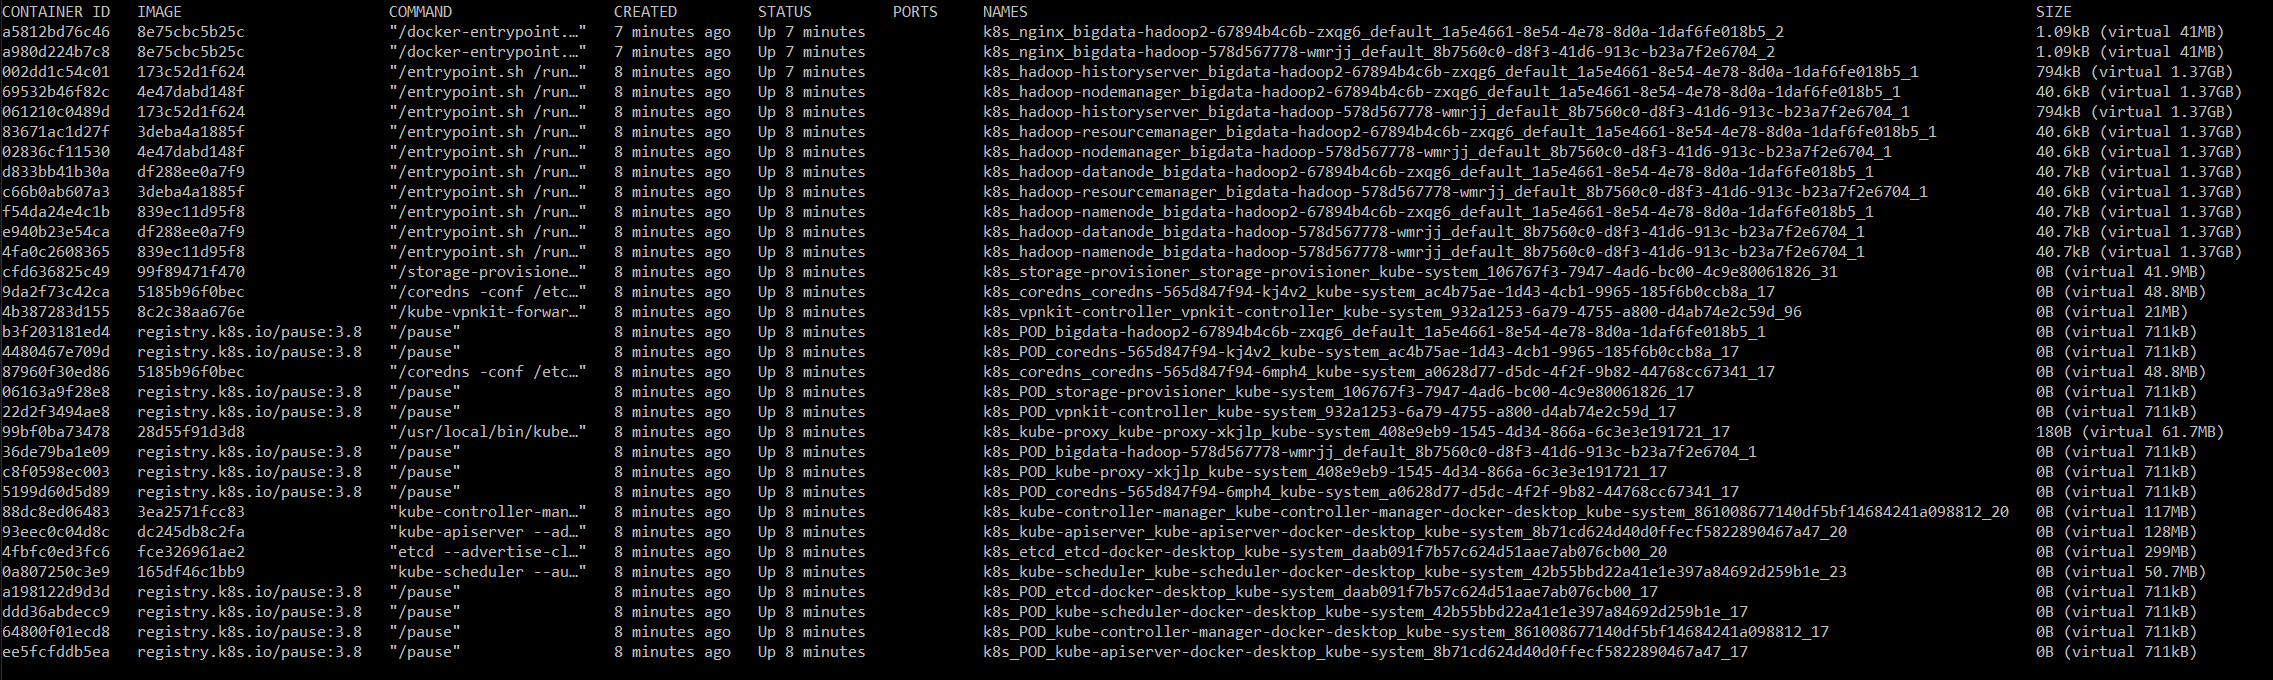
\includegraphics[scale=0.4]{Hadoop 2 pods resource usage size.png}
    \caption{TODO}
\end{figure}

\begin{figure}
    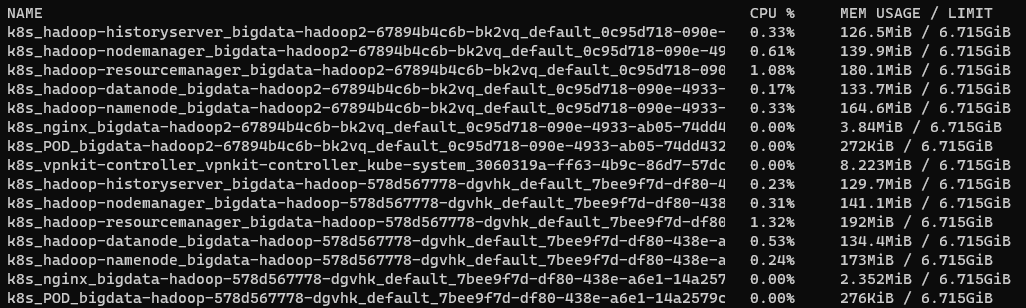
\includegraphics[scale=0.4]{Hadoop 2 pods resource usage.png}
    \caption{TODO}
\end{figure}

\begin{figure}
    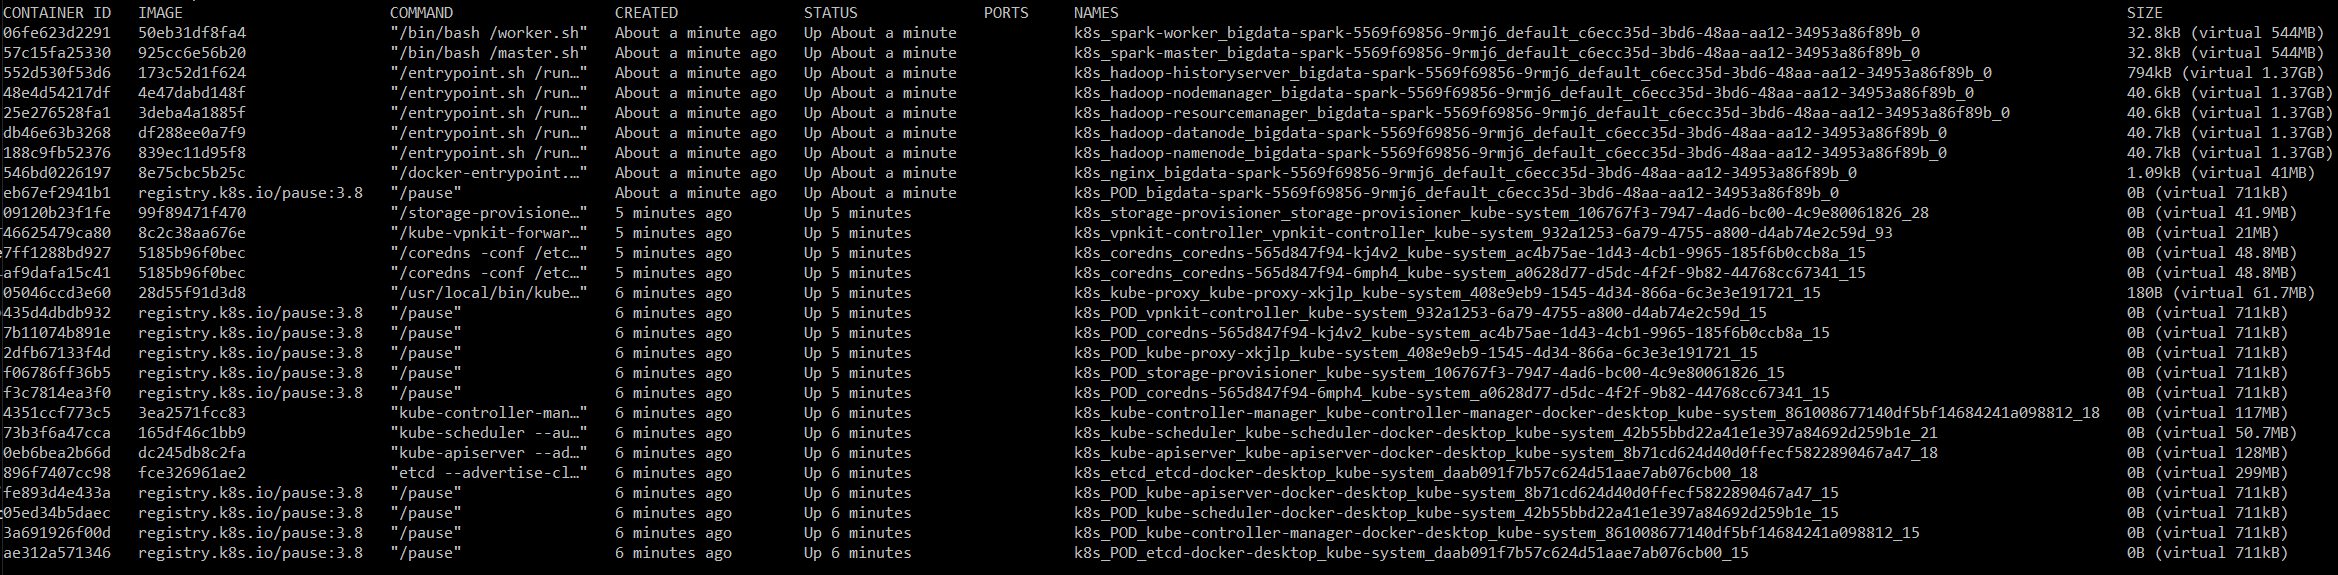
\includegraphics[scale=0.4]{Hadoop and Spark resource usage size.png}
    \caption{TODO}
\end{figure}

\begin{figure}
    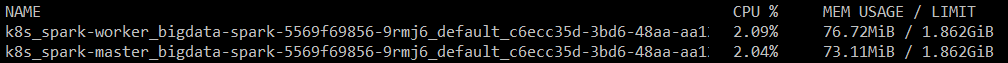
\includegraphics[scale=0.4]{Hadoop and Spark resource usage.png}
    \caption{TODO}
\end{figure}

\begin{figure}
    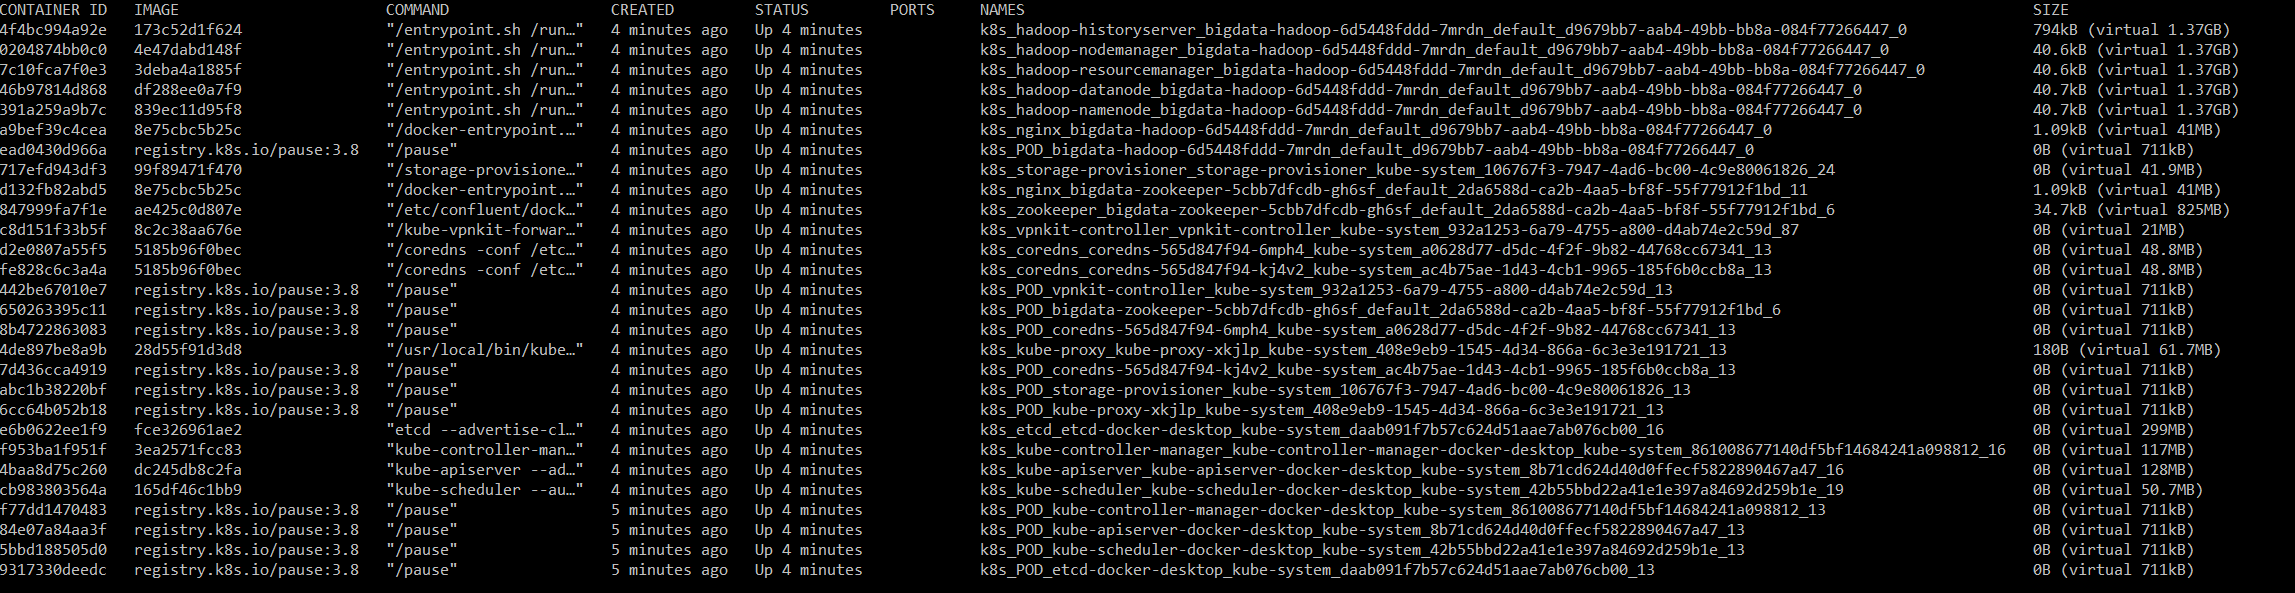
\includegraphics[scale=0.4]{Hadoop resource usage size.png}
    \caption{TODO}
\end{figure}

\begin{figure}
    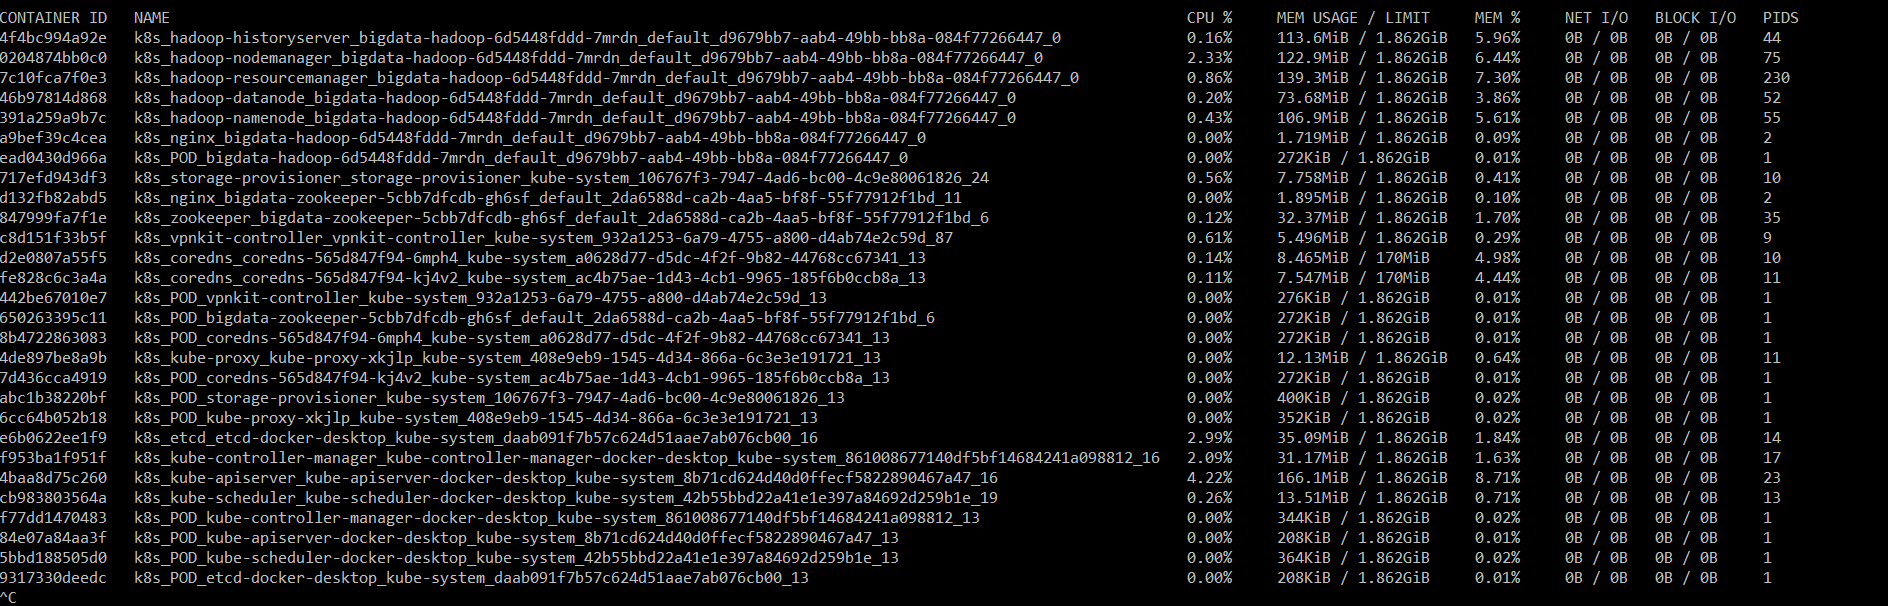
\includegraphics[scale=0.4]{Hadoop resource usage.png}
    \caption{TODO}
\end{figure}

\begin{figure}
    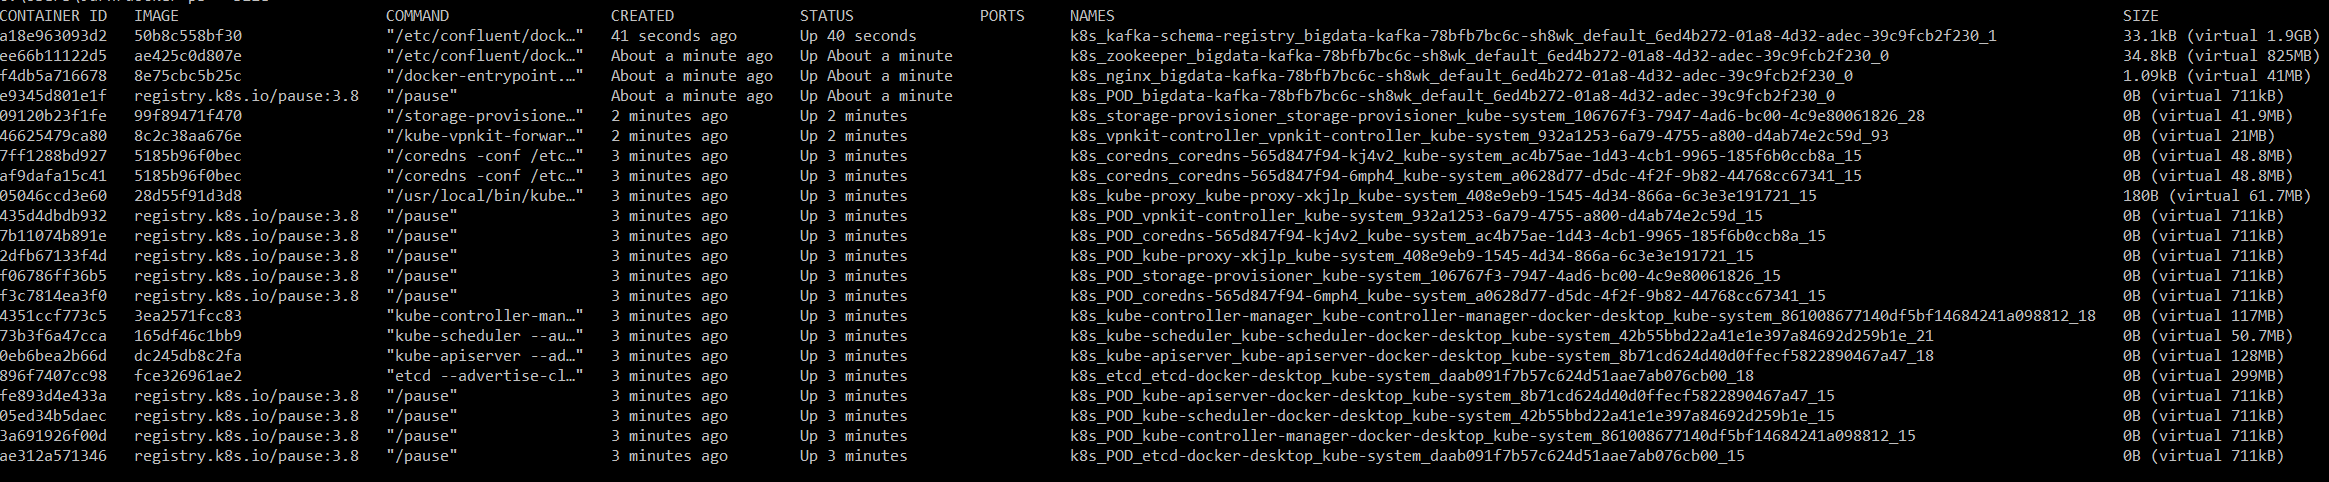
\includegraphics[scale=0.4]{Kafka resource usage size.png}
    \caption{TODO}
\end{figure}

\begin{figure}
    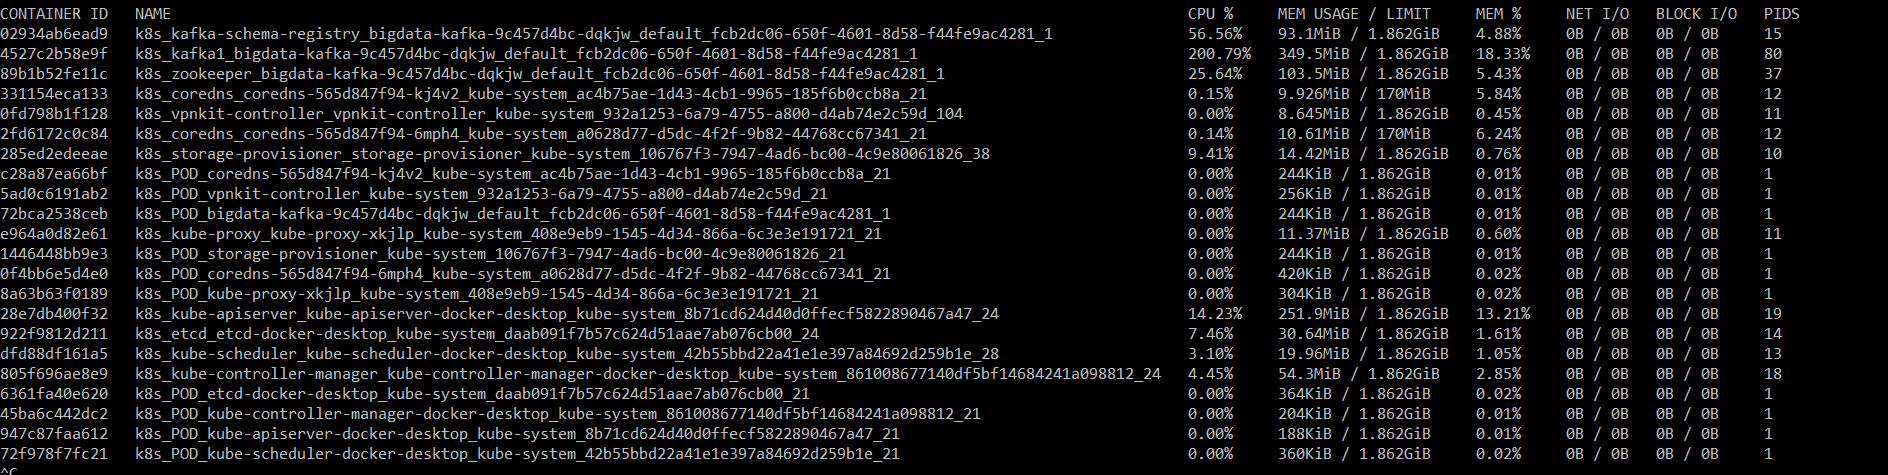
\includegraphics[scale=0.4]{Kafka resource usage.png}
    \caption{TODO}
\end{figure}


% Voeg hier je eigen hoofdstukken toe die de ``corpus'' van je bachelorproef
% vormen. De structuur en titels hangen af van je eigen onderzoek. Je kan bv.
% elke fase in je onderzoek in een apart hoofdstuk bespreken.

%\input{...}
%\input{...}
%...

%%=============================================================================
%% Conclusie
%%=============================================================================

\chapter{Conclusie}%
\label{ch:conclusie}

% TODO: Trek een duidelijke conclusie, in de vorm van een antwoord op de
% onderzoeksvra(a)g(en). Wat was jouw bijdrage aan het onderzoeksdomein en
% hoe biedt dit meerwaarde aan het vakgebied/doelgroep? 
% Reflecteer kritisch over het resultaat. In Engelse teksten wordt deze sectie
% ``Discussion'' genoemd. Had je deze uitkomst verwacht? Zijn er zaken die nog
% niet duidelijk zijn?
% Heeft het onderzoek geleid tot nieuwe vragen die uitnodigen tot verder 
%onderzoek?

\lipsum[76-80]



%---------- Bijlagen -----------------------------------------------------------

\appendix

\chapter{Onderzoeksvoorstel}

Het onderwerp van deze bachelorproef is gebaseerd op een onderzoeksvoorstel dat vooraf werd beoordeeld door de promotor. Dat voorstel is opgenomen in deze bijlage.

%% TODO: 
%\section*{Samenvatting}

% Kopieer en plak hier de samenvatting (abstract) van je onderzoeksvoorstel.

% Verwijzing naar het bestand met de inhoud van het onderzoeksvoorstel
%---------- Inleiding ---------------------------------------------------------

\section{Introductie}%
\label{sec:introductie}

In het kader van de opleiding Toegepaste Informatica HoGent worden de Big Data frameworks Hadoop, Spark en Kafka gebruikt. Het is niet eenvoudig om deze software te installeren op de laptop van de student, hiermee gaat kostbare leertijd verloren.
De doelstelling is uit te zoeken of containertechnologie kan gebruikt worden om deze verschillende applicaties te installeren op het VIC\footnote{HoGent Virtual IT Company}, rekening houdende met vereisten als efficiënt gebruik van hulpbronnen, beveiliging en stabiliteit (gebruikers van elkaar afschermen), schaalbaarheid en logging.
De bedoeling is dat de resultaten van dit onderzoek in de volgende jaren kunnen gebruikt worden om de lessen van het vak ``Big Data Processing'' te faciliteren.

%---------- Stand van zaken ---------------------------------------------------

\section{State-of-the-art}%
\label{sec:state-of-the-art}
Hadoop en Spark, beide ontwikkeld door de Apache Software Foundation, zijn veelgebruikte open-source frameworks voor big data- architecturen. Elk framework bevat open-source technologieën die big data sets voorbereiden, beheren en verwerken.
Beiden verdelen de processing van grote data sets over een cluster van computernodes.
Hadoop word vaak als basis voor een big data architecture gebruikt terwijl Spark sneller MapReduce doet door RAM te gebruiken en daardoor ook sneller is voor kleinere datasets die volledig in het RAM geheugen passen. Kafka word gebruikt naast Hadoop om real-time data streams te verzamelen.(\autocite{Hadoop} \autocite{Spark} \autocite{Kafka})
Hadoop, Spark en Kafka worden al samen gebruikt volgens \autocite{Holmes2012}:
'In this situation, you'd use Kafka to both land data on Hadoop and provide a feed into a real-time data-streaming system such as Storm or Spark Streaming, which you could then use to perform near-real-time computations.' en \autocite{Leang2019}:
'one of the more significant findings to emerge from this study is that the integration of the Hadoop system especially Apache Kafka and Apache Spark enhances the performance and accuracy of data storing, processing, and securing in the manufacturing environment.'

Er is informatie te vinden over het gebruik van Docker om verschillende combinaties van 2 van de 3 frameworks te installeren maar niks over alle 3 samen, zeker niet met de requirements die wij willen onderzoeken. 

% Voor literatuurverwijzingen zijn er twee belangrijke commando's:
% \autocite{KEY} => (Auteur, jaartal) Gebruik dit als de naam van de auteur
%   geen onderdeel is van de zin.
% \textcite{KEY} => Auteur (jaartal)  Gebruik dit als de auteursnaam wel een
%   functie heeft in de zin (bv. ``Uit onderzoek door Doll & Hill (1954) bleek
%   ...'')

%---------- Methodologie ------------------------------------------------------
\section{Methodologie}%
\label{sec:methodologie}
Het onderzoek wordt gestart met een studie van de installaties van Hadoop, Spark en Kafka, en hun configuratie en onderlinge samenhang.
Met een focus op de requirements zoals vermeld in de Introductie, zoals bijvoorbeeld beveiliging en schaalbaarheid.
Startpunt is de documentatie op de website van de verschillende tools. Ik verwacht ook relevante artikels op het web te vinden, met gedetailleerde voorbeelden uit de praktijk.
Een bron van informatie is zeker ook de cursus van het vak ``Big Data Processing'', om een goed zicht te hebben op de manier waarop de tools worden gebruikt.

Om de installatievereisten te vertalen naar containertechnologie als Virtual Machines, Docker, Docker Compose en Kubernetes, volgt er ook een studie van deze, opnieuw met als startpunt de website van de verschillende tools.
Hierbij wordt er rekening gehouden met de mogelijkheden en technologieën zoals vandaag gebruikt in de infrastruktuur van het VIC. Om hierover meer te leren denk ik gebruik te maken van cursussen van VIC gerelateerde vakken van de richting OPS.

%---------- Verwachte resultaten ----------------------------------------------
\section{Verwacht resultaat, conclusie}%
\label{sec:verwachte_resultaten}
Ik verwacht dat het mogelijk zal zijn om de installatie en configuratie van de 3 frameworks te automatiseren, gebruik makende van Docker, Docker Compose en Kubernetes.
De details hiervan zullen beschreven worden in mijn Bachelorproef, samen met voorbeelden van scripts, configuratie files en andere nodige artifacts om de installaties voor het vak ``Big Data Processing'' te faciliteren.


\chapter{Docker compose}

\input{docker-compose.yaml}

%%---------- Andere bijlagen --------------------------------------------------
% TODO: Voeg hier eventuele andere bijlagen toe. Bv. als je deze BP voor de
% tweede keer indient, een overzicht van de verbeteringen t.o.v. het origineel.
%\input{...}

%%---------- Backmatter, referentielijst ---------------------------------------

\backmatter{}

\setlength\bibitemsep{2pt} %% Add Some space between the bibliograpy entries
\printbibliography[heading=bibintoc]

\end{document}
